% !TEX program = xelatex
% !BIB program = bibtex
\documentclass[10pt,a4paper]{article}

\usepackage{fontspec}
\defaultfontfeatures{Ligatures=TeX}
\setmainfont{TeX Gyre Termes}
\setsansfont{TeX Gyre Heros}
\setmonofont{TeX Gyre Cursor}

\usepackage[a4paper,margin=20mm,headheight=14pt]{geometry}
\usepackage{microtype}
\usepackage{setspace}
\setstretch{1.025}
\setlength{\emergencystretch}{2em}
\usepackage{amsmath,amssymb,bm}
\usepackage{booktabs,tabularx,array,longtable,multirow}
\usepackage{graphicx}
\usepackage{tikz}
\usetikzlibrary{arrows.meta,positioning,fit,calc,shapes.geometric,backgrounds,matrix}
\usepackage{float}
\usepackage{placeins}
\usepackage{xcolor}
\usepackage{enumitem}
\usepackage{siunitx}
\usepackage[font=small,labelfont=bf]{caption}
\usepackage[numbers,sort&compress]{natbib}
\usepackage{hyperref}
\usepackage[nameinlink,noabbrev]{cleveref}
\usepackage{fancyhdr}

\definecolor{reviewblue}{HTML}{1F5A7A}
\definecolor{reviewteal}{HTML}{267D78}
\definecolor{revieworange}{HTML}{C56A2D}
\definecolor{reviewred}{HTML}{A4473D}
\definecolor{reviewgray}{HTML}{59636E}
\definecolor{reviewlight}{HTML}{EEF4F6}
\definecolor{reviewwarm}{HTML}{FBF2E8}

% Author and institutional metadata shared by the review title block and PDF metadata.
\newcommand{\ProposalTitle}{BiCG-Rep: Observation-Grounded Dynamic Bimanual Contact-Flow Representations for Load Transfer and Tool Manipulation}
\newcommand{\ProposalAuthor}{XU XIANGYU}
\newcommand{\DegreeProgramme}{Master's Degree Programme}
\newcommand{\DepartmentName}{PINE Lab / School of Electrical and Electronic Engineering}
\newcommand{\InstitutionName}{Nanyang Technological University}
\newcommand{\SupervisorName}{Liu Haichao, Wang Ziwei}
\newcommand{\SubmissionDate}{August 2026}


\hypersetup{
  colorlinks=true,
  linkcolor=reviewblue,
  citecolor=reviewteal,
  urlcolor=reviewblue,
  pdftitle={Structured Tactile Representations for Bimanual Contact-Rich Manipulation},
  pdfauthor={\ProposalAuthor}
}

\setlist[itemize]{leftmargin=*,topsep=3pt,itemsep=2pt}
\setlist[enumerate]{leftmargin=*,topsep=3pt,itemsep=2pt}
\setlength{\tabcolsep}{4.5pt}
\renewcommand{\arraystretch}{1.14}
\newcolumntype{Y}{>{\raggedright\arraybackslash}X}
\newcolumntype{C}{>{\centering\arraybackslash}X}
\newcolumntype{P}[1]{>{\raggedright\arraybackslash}p{#1}}
\newcommand{\yes}{\textcolor{reviewteal}{\ensuremath{\checkmark}}}

\pagestyle{fancy}
\fancyhf{}
\fancyhead[L]{Structured Tactile Representations for Bimanual Manipulation}
\fancyhead[R]{\thepage}
\renewcommand{\headrulewidth}{0.3pt}

\title{\bfseries\color{reviewblue}Structured Tactile Representations for Bimanual Contact-Rich Manipulation:\\[2mm]
\large Task Topologies, Physical Grounding, and Evidence}
\author{\ProposalAuthor\\[-1mm]\small \DepartmentName\\\small \InstitutionName}
\date{Curated scoping-review draft --- corpus updated 30 August 2026;\\
core full-text coding completed 13 August 2026}

\begin{document}
\maketitle

\begin{abstract}
Tactile learning has progressed from task-specific force features to
self-supervised encoders, cross-sensor foundation models, spatial anchoring,
contact fields, and graph-based dynamics. In parallel, bimanual manipulation has
advanced through large-scale simulation, imitation, human-motion retargeting,
and increasingly capable real systems. The intersection remains conceptually
fragmented: a representation that recognizes local contact is not necessarily
one that explains how load, slip, and constraint changes propagate between two
hands through an object, tool, workpiece, or environment. This paper presents a
curated scoping review of 91 archived records spanning tactile representation,
bimanual coordination and handover, relational and physics-informed learning,
tool--workpiece control, and datasets. Ninety scholarly works enter the
  narrative synthesis; publication status is kept explicit because the rapidly
  moving 2025--2026 frontier contains many preprints and programme-listed papers.
  The archive-wide evidence map is complemented by full-text precision coding of
  a purposive 30-paper core (19 Level A and 11 Level B records), with located
  evidence separated from author claims and reviewer inference.

We organize the literature along six independent axes: task/contact topology,
representation scale, structural prior, supervision source, deployment
observability, and strength of evaluation evidence. This organization exposes
three recurring gaps. First, most tactile encoders model local or temporal
content without testing whether cross-interface load paths are recoverable.
Second, graph and contact-structured methods often obtain their topology from
kinematics, simulator state, or predefined edges rather than infer it from
deployable observations. Third, bimanual studies commonly report task success
  without matched-budget representation baselines, transition-level diagnostics,
  or topology-level out-of-distribution tests. None of the 30 core papers tested
  strict held-out contact-topology transfer under a deployment-observable inference
  protocol. Handover provides a controlled load-transfer laboratory, while
  cooperative tool--workpiece manipulation adds a harder multi-hop topology. Tool
  use itself is established, but matched studies of observation-grounded
  cross-hand load flow remain comparatively sparse in the mapped corpus. We
  conclude with an evidence-based
research agenda centred on observation-grounded structure, interface-level
prediction, uncertainty, causal interventions, and transfer across contact
topologies. The review does not argue that graphs are intrinsically superior;
it specifies the experiments required to establish when explicit structure is
useful.
\end{abstract}

\noindent\textbf{Keywords:} tactile representation learning; bimanual manipulation;
contact-rich robotics; dynamic contact graphs; handover; load transfer; tool use;
visuo-tactile learning; scoping review.

\vspace{2mm}
\noindent\fcolorbox{reviewblue}{reviewlight}{%
\parbox{0.965\linewidth}{\small
\textbf{Scope statement.} This is a reproducible, curated scoping review of the
local research archive, not a PRISMA-complete systematic review or a quantitative
meta-analysis. Counts describe the archived corpus and should not be interpreted
as publication-rate estimates for the entire field.}}

\section{Introduction}
\label{sec:introduction}

Contact-rich manipulation is partially observable in a particularly consequential
way. Vision can estimate object pose before contact, but it cannot directly reveal
the pressure redistribution that precedes slip, the direction of an incipient
constraint, or whether an apparently stable object is actually supported by the
left hand, the right hand, a tool, or the environment. Tactile sensing reduces
this ambiguity at an individual interface. Bimanual manipulation then creates a
second problem: the controller must relate several local interfaces whose states
are coupled through shared rigid-body motion, compliance, friction, and changes
in contact topology.

The distinction is easiest to see in a handover. Before transfer, the giver bears
most of the load. During dual contact, the same object couples both hands, and a
safe release depends on the receiver's support rather than on giver touch alone.
After release, the cross-hand path disappears. A representation that concatenates
two tactile streams can, in principle, approximate this mapping, but it does not
state which interfaces interact, which entity mediates the interaction, or why
the mapping should transfer to a new grasp topology. Conversely, a graph can name
the interfaces, yet a graph whose edges are fixed or supplied by a simulator does
not solve contact inference at deployment.

Recent work makes this review timely. Large tactile pretraining systems learn
sensor-robust local features from video-based touch, robot play, and multimodal
alignment~\cite{guzey2023tdex,higuera2025sparsh,yang2024unitouch,feng2025anytouch,zhao2024t3}.
Spatially anchored and cross-modal models seek to place touch in a geometric or
temporal context~\cite{huang2025sata,heng2025vitacformer}. Relational models use
graphs for tactile arrays, learned dynamics, morphology, and contact
physics~\cite{funabashi2022distributed,yang2023tacgnn,ai2024robopack,battaglia2016interaction,sanchez2020gns}.
At the same time, bimanual policy learning has expanded from simulated suites to
human demonstrations and real systems~\cite{chen2022bidexhands,grannen2023stabilize,shaw2024bidex,jiang2024dexmimicgen,li2025maniptrans}.
The 2026 frontier further includes tactile-reactive bimanual control, whole-hand
benchmarks, morphology-aware tactile policies, contact-anchored control, and
tool-oriented contact fields~\cite{niu2026trex,yuan2026ftp1,huang2026htbench,cui2026contactanchored,ma2026semanticcontact}.

The two late-August surveillance updates sharpen this frontier. Hierarchical
tactile world models now separate contact, deformation, and slip prediction;
sequential visuo-tactile learning uses temporal alignment and training-time
privileged posteriors; and physics-aware sensing explicitly models object
properties or time-dependent viscoelastic relaxation
~\cite{xue2026hitacwam,xu2026vtmuse,liu2026vitacphys,wang2026relaxation}.
Meanwhile, structured cloth dynamics combine a mesh prior with a learned global
residual~\cite{wang2026meshpriordit}. These advances strengthen the relevant
alternatives to a contact graph: a valid comparison is no longer ``graph versus
concatenation'', but observation-matched structured priors, predictive temporal
models, and residual global models. None of these additions, however, directly
demonstrates observation-grounded cross-hand load topology.

The September--early-October catch-up changes the wording of the gap itself.
BiView-Touch provides direct offline human cross-hand tactile representation
evidence, while temporal tactile encoding with compliance provides a strong real
bimanual handover control baseline~\cite{liang2026biviewtouch,marra2026temporaltactilehandover}.
CADeT additionally shows observation-grounded transmission-mode inference and
physical probing in visually observed tissue manipulation~\cite{hu2026cadet}.
These are positive results at different links of the evidence chain. The remaining
question is their combination with independently validated robotic cross-hand
loads, matched structural controls, and topology-defined transfer, rather than
whether relational touch or inferred interaction modes exist at all.

These advances do not yet answer a shared representation question:

\begin{quote}
\emph{When does an explicit, observation-grounded model of contact topology and
load propagation improve bimanual perception or control over an equally capable
unstructured temporal model?}
\end{quote}

This formulation avoids two shortcuts. The first is to equate tactile input with
physical grounding. A policy may receive fingertip forces while depending on
object state, simulator contacts, or a future reference trajectory. The second is
to equate a graph architecture with a scientific contribution. Generic relational
learning is well established~\cite{battaglia2016interaction,wang2018nervenet,ying2021graphormer};
the contribution must lie in what the nodes and edges mean, how they can be
inferred, which physical quantities they predict, and which counterfactual tests
they survive.

\subsection{Review objectives and contributions}

This review integrates literatures that are often treated separately: local
tactile representation learning, structured contact and dynamics models,
bimanual manipulation and handover, cooperative tool use, and benchmark design.
Its contributions are fourfold.

\begin{enumerate}
  \item It introduces an orthogonal taxonomy that separates task topology,
  representation level, structural prior, supervision source, deployment
  observability, and evaluation evidence. This prevents a method from appearing
  physically grounded solely because it uses tactile inputs or graph layers.

  \item It distinguishes \emph{local contact representation} from
  \emph{cross-interface coordination representation}. The former encodes what a
  sensor sees; the latter must preserve which interfaces are coupled, how support
  is redistributed, and how this relation changes over time.

  \item It positions quasi-static handover and cooperative tool--workpiece tasks
  as complementary experimental topologies. Handover isolates support transfer;
  tool use tests multi-hop, role-asymmetric coupling without making an unsupported
  claim that the area is empty.

  \item It converts broad calls for ``better physical representations'' into a
  falsifiable evaluation programme: matched observation and parameter budgets,
  oracle, inferred, and random structure comparisons; contact-transition metrics;
  object-, session-, and contact-sequence-level splits; uncertainty calibration;
  and targeted interventions.
\end{enumerate}

The intended outcome is not a leaderboard. Sensor form factors, embodiments,
training data, task semantics, and success definitions vary too much for a valid
pooled effect estimate. Instead, the review identifies which claims can be made
from current evidence and which experiments are still needed.

\subsection{Terminology}

We use \emph{tactile observation} for a measured taxel array, tactile image,
deformation field, event stream, or calibrated interface force/torque signal.
Simple simulator contact flags and full object state are called \emph{privileged
contact variables} unless the deployment system measures them. \emph{Contact
topology} denotes the set of active interfaces between hands, objects, tools,
workpieces, and the environment. \emph{Load path} denotes a sequence of such
interfaces through which forces and moments are transmitted. \emph{Structured
representation} covers graphs, contact fields, object-centric frames, spatial
anchors, and other models that state relations beyond token order. These terms
describe information and assumptions, not a preferred neural architecture.

\section{Review Method and Corpus}
\label{sec:method}

\subsection{Review design}

The study is a curated scoping review. Scoping review methodology is appropriate
when concepts, evidence types, and evaluation practices are heterogeneous and the
goal is to map a field rather than estimate one pooled treatment
effect~\cite{tricco2018prismascr}. The accompanying \texttt{review\_protocol.md}
records the scope, eligibility criteria, evidence fields, update procedure, and
limitations. The machine-readable \texttt{evidence\_matrix.csv} is generated from
the workspace manifest by a versioned script; rule-assisted annotations remain
subject to manual audit. A second evidence layer, stored in
\texttt{precision\_annotations/}, contains full-text precision coding and an
individual evidence card for each of 30 purposively selected core papers.

The corpus was frozen on 12 August 2026. It began from a decision-oriented archive
assembled for research planning and was expanded around five intersecting areas:
(i) tactile and visuo-tactile representation learning; (ii) bimanual dexterous
manipulation and handover; (iii) graph, contact-field, object-centric, and
physics-informed models; (iv) tool--workpiece contact control; and (v) datasets
and benchmarks. Backward and forward chaining was used selectively for landmark
and directly competing works. Author project pages, arXiv records, official
conference programmes, proceedings pages, and publisher records were used to
disambiguate status.

The current draft follows the reporting intent of PRISMA-ScR but does not claim
formal PRISMA compliance. It does not reproduce database-by-database search
strings, use dual independent screening, or apply a validated cross-design
risk-of-bias tool. These omissions matter: the numerical corpus summary is an
audit of this archive, not a bibliometric description of the whole field.

\subsection{Two-layer evidence design}

The archive-wide layer covers all 74 records. Title, abstract, publication and
artifact metadata, and selectively consulted full text support eligibility,
status accounting, and coarse six-axis coding. This layer provides breadth but
is not used as if every row were an independently extracted full-text study.

The precision layer was completed on 13 August 2026 for 30 papers selected for
their decision relevance rather than for statistical representativeness. The
subset comprises 19 Level A records, coded through full text plus available
artifact or code evidence, and 11 Level B records, coded through full-text method
and evidence analysis. It covers direct system competitors, executable
benchmarks, graph and relational models, contact fields and anchors, mechanics
and control references, tool-use systems, and candidate local tactile encoders.
Each record distinguishes (i) the authors' claim, (ii) evidence located in the
paper or artifact, and (iii) reviewer inference. It also separates deployment
inputs from training-only privilege and codes object, sensor, embodiment, and
contact-topology OOD as different claims. All 30 cards contain evidence locations;
the procedure is full-text evidence coding, not independent reproduction.

\begin{table}[t]
\centering
\caption{Review questions and the evidence required to answer them.}
\label{tab:rqs}
\begin{tabularx}{\linewidth}{P{0.08\linewidth} Y Y}
\toprule
\textbf{RQ} & \textbf{Question} & \textbf{Primary evidence fields} \\
\midrule
RQ1 & What must be preserved for bimanual contact-rich manipulation? & Task topology, predicted quantities, temporal horizon, interface identity. \\
RQ2 & How is touch organized across sensors, bodies, entities, and time? & Representation scale, tokenization, spatial frame, structural prior. \\
RQ3 & Is the structure available at deployment? & Sensor inputs, privileged state, inferred versus supplied topology, future reference. \\
RQ4 & How is usefulness demonstrated? & Baselines, split unit, probes, control metrics, OOD tests, interventions, uncertainty. \\
RQ5 & Where are the actionable gaps? & Missing topology--method cells, weak evidence links, unavailable labels or benchmarks. \\
\bottomrule
\end{tabularx}
\end{table}

\subsection{Eligibility and coding}

Scholarly work was included when it materially addressed robot touch,
contact-state or dynamics estimation, tactile-informed control, bimanual
coordination, handover, tool use, or an enabling benchmark. Generic graph and
physics-learning papers were included only where their formulation directly
informs relational contact modelling. A community tactile-data index was retained
as a resource record but excluded from study-level synthesis. Duplicate versions
were represented by the most informative accessible record, with publication
status documented rather than silently upgraded.

Each record was coded along six axes:

\begin{enumerate}
  \item \textbf{Task/contact topology:} single interface, multi-finger hand,
  two hands sharing an object, sequential/overlapping handover, hand--tool--
  environment, or hand--tool--workpiece--hand.
  \item \textbf{Representation scale:} local patch, finger/link, hand,
  object/interface, cross-entity relation, or trajectory-level latent.
  \item \textbf{Structural prior:} token order, kinematics, object-centric
  coordinates, spatial anchors, contact fields/modes, or graph connectivity.
  \item \textbf{Supervision source:} instance discrimination, reconstruction,
  cross-modal alignment, action-conditioned prediction, simulator labels,
  force/pose measurement, or task reward.
  \item \textbf{Deployment observability:} directly sensed, perception-derived,
  training-only privilege, or unavailable future reference.
  \item \textbf{Evidence:} representation probe, open-loop prediction,
  closed-loop control, real transfer, OOD topology, intervention, and uncertainty.
\end{enumerate}

The axes are kept separate because they answer different validity questions.
A real-robot paper can use weak splits; a simulation paper can isolate a causal
mechanism cleanly; a high-capacity pretrained encoder can be deployable but offer
no cross-interface structure; and a physically interpretable graph can depend on
unavailable state.

\subsection{Corpus accounting and status discipline}

The archive contains 74 records: 12 core or directly competing systems, 19
bimanual and handover works, 16 tactile-representation works, 13 graph, physics,
and contact works, eight tool--workpiece works, and six dataset or benchmark records. Sixty-nine
PDFs are now locally validated; five records retain authoritative
source links without a local PDF. Seventy-three scholarly studies enter the
narrative synthesis and one community index is resource-only.

After correcting several manifest entries for identifiable formal proceedings,
the evidence matrix records 46 peer-reviewed works, eight works listed as accepted
or on an official programme, 19 preprints or author-claim records, and one
community resource. ``Accepted'' is not treated as equivalent to a final
publisher record. In particular, rapidly emerging 2026 works are discussed as
directions and evidence, not as settled consensus.

\begin{figure}[t]
\centering
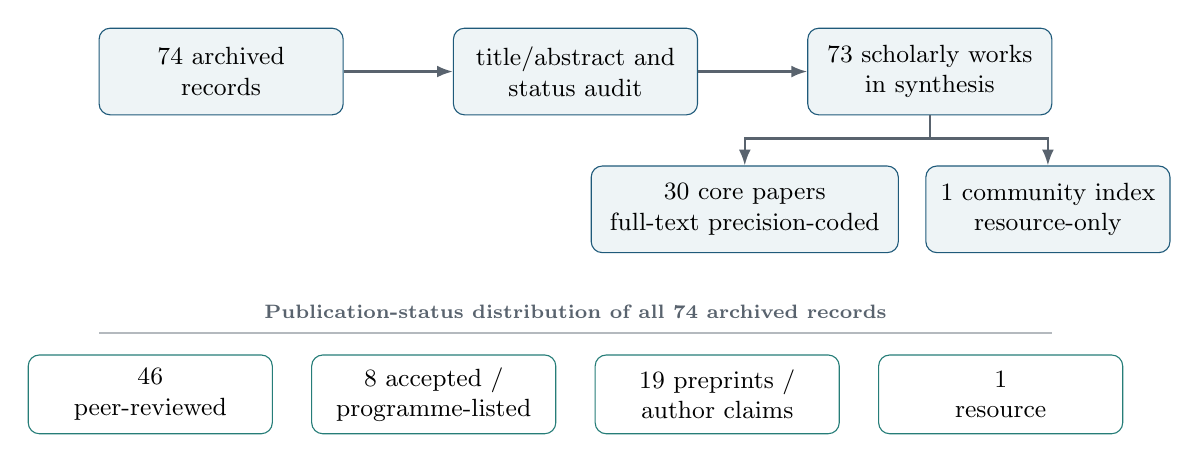
\begin{tikzpicture}[
  box/.style={draw=reviewblue, rounded corners, fill=reviewlight, minimum width=31mm,
              minimum height=11mm, align=center, font=\small},
  status/.style={draw=reviewteal, rounded corners, fill=white, minimum width=31mm,
                 minimum height=10mm, align=center, font=\small},
  arr/.style={-{Latex[length=2mm]}, thick, draw=reviewgray}
]
\node[box] (archive) at (0,3.1) {74 archived\\records};
\node[box] (screen) at (4.5,3.1) {title/abstract and\\status audit};
\node[box] (synth) at (9.0,3.1) {73 scholarly works\\in synthesis};
\node[box, minimum width=39mm] (precision) at (6.65,1.35)
  {30 core papers\\full-text precision-coded};
\node[box] (resource) at (10.5,1.35) {1 community index\\resource-only};
\draw[arr] (archive) -- (screen);
\draw[arr] (screen) -- (synth);
\coordinate (fork) at (9.0,2.25);
\draw[arr] (synth.south) -- (fork) -| (precision.north);
\draw[arr] (fork) -| (resource.north);

\node[font=\scriptsize\bfseries, text=reviewgray] at (4.5,0.05)
  {Publication-status distribution of all 74 archived records};
\draw[reviewgray!45, thin] (-1.55,-0.22) -- (10.55,-0.22);
\node[status] (peer) at (-0.9,-1.0) {46\\peer-reviewed};
\node[status] (accept) at (2.7,-1.0) {8 accepted /\\programme-listed};
\node[status] (pre) at (6.3,-1.0) {19 preprints /\\author claims};
\node[status] (res) at (9.9,-1.0) {1\\resource};
\end{tikzpicture}
\caption{Two-layer corpus flow and publication-status accounting. All 74 records
receive archive-wide screening and coarse coding; the purposive 30-paper subset
receives full-text precision coding. Counts describe the curated archive, not the
global literature.}
\label{fig:corpus}
\end{figure}

\subsection{Synthesis strategy}

The synthesis is concept-centric rather than paper-by-paper. Representative
methods are compared within the same information problem, and negative space is
made explicit: for example, a work may demonstrate cross-sensor transfer without
testing cross-hand load inference, or closed-loop bimanual success without an
explicit tactile representation ablation. No pooled accuracy or success rate is
reported because task definitions, sensor density, action spaces, data scale,
embodiments, and test splits are not commensurate. Descriptive counts from the
precision subset are reported only when the denominator and coding rule are
explicit. In particular, zero of the 30 core papers evaluated strict held-out
contact-topology OOD under deployment-observable inference. Here ``strict'' means
that the participant/edge structure itself is held out; unseen objects, contact
modes within a fixed structure, tool geometry, or semantic task compositions do
not qualify. Claims that a specific intersection is comparatively sparse are
stated as inferences from the mapped corpus rather than field-wide publication
counts.

\section{Task Topologies and Representation Requirements}
\label{sec:topologies}

\subsection{Why topology is a more useful organizing variable than task name}

Task labels conceal important physical differences. ``Handover'' can mean a
quasi-static transfer with simultaneous support, a dynamic throw--catch event,
or a robot--human release triggered by pull and slip. ``Tool use'' can mean one
hand moving a rigid tool against a fixed environment, one hand stabilizing a
workpiece while the other acts, or both hands jointly holding the same tool.
These variants demand different information even when their semantic label is
the same. A representation-oriented review should therefore begin with the
active interfaces and their changes.

Let the task at time $t$ contain entities
$\mathcal{V}_t=\{H_L,H_R,O_1,\ldots,T_1,\ldots,W,E\}$ for left and right hands,
objects, tools, a workpiece, and environment. The physical contact topology is
$\mathcal{G}^{c}_t=(\mathcal{V}_t,\mathcal{E}^{c}_t)$, where an edge represents
an active load-bearing or constraint-producing interface. This notation does
not require the model itself to be a graph neural network. It provides a neutral
way to ask whether the observation history $o_{1:t}$ contains enough information
to infer the relevant interfaces and their direction-dependent effects.

\begin{figure}[t]
\centering
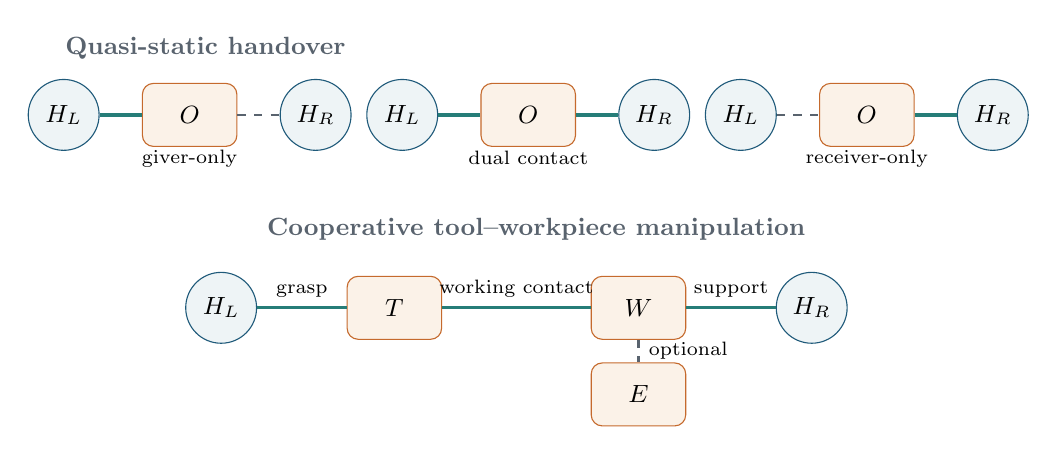
\begin{tikzpicture}[
  entity/.style={circle, draw=reviewblue, fill=reviewlight, minimum size=9mm,
                 font=\small\bfseries},
  tool/.style={rectangle, rounded corners, draw=revieworange, fill=reviewwarm,
               minimum width=12mm, minimum height=8mm, font=\small\bfseries},
  contact/.style={line width=1.2pt, draw=reviewteal},
  inactive/.style={line width=0.8pt, draw=reviewgray, dashed},
  phase/.style={font=\small\bfseries, text=reviewgray}
]
% handover phases
\node[phase] at (1.8,2.65) {Quasi-static handover};
\node[entity] (gl) at (0,1.8) {$H_L$};
\node[tool] (o1) at (1.6,1.8) {$O$};
\node[entity] (gr) at (3.2,1.8) {$H_R$};
\draw[contact] (gl)--(o1);
\draw[inactive] (o1)--(gr);
\node[font=\scriptsize] at (1.6,1.25) {giver-only};

\node[entity] (dl) at (4.3,1.8) {$H_L$};
\node[tool] (o2) at (5.9,1.8) {$O$};
\node[entity] (dr) at (7.5,1.8) {$H_R$};
\draw[contact] (dl)--(o2);
\draw[contact] (o2)--(dr);
\node[font=\scriptsize] at (5.9,1.25) {dual contact};

\node[entity] (rl) at (8.6,1.8) {$H_L$};
\node[tool] (o3) at (10.2,1.8) {$O$};
\node[entity] (rr) at (11.8,1.8) {$H_R$};
\draw[inactive] (rl)--(o3);
\draw[contact] (o3)--(rr);
\node[font=\scriptsize] at (10.2,1.25) {receiver-only};

% tool workpiece
\node[phase] at (6.0,0.35) {Cooperative tool--workpiece manipulation};
\node[entity] (hl2) at (2.0,-0.65) {$H_L$};
\node[tool] (tool2) at (4.2,-0.65) {$T$};
\node[tool] (work) at (7.3,-0.65) {$W$};
\node[entity] (hr2) at (9.5,-0.65) {$H_R$};
\draw[contact] (hl2)-- node[above,font=\scriptsize] {grasp} (tool2);
\draw[contact] (tool2)-- node[above,font=\scriptsize] {working contact} (work);
\draw[contact] (work)-- node[above,font=\scriptsize] {support} (hr2);
\node[tool] (env) at (7.3,-1.75) {$E$};
\draw[inactive] (work)-- node[right,font=\scriptsize] {optional} (env);
\end{tikzpicture}
\caption{Two complementary topology families. Handover changes which hand
supports a shared object; tool--workpiece manipulation introduces a longer,
role-asymmetric load path. Dashed edges are inactive or optional.}
\label{fig:topologies}
\end{figure}

\subsection{Six topology families}

\paragraph{Local single-interface contact.}
The simplest case associates a tactile patch with local geometry, force, slip,
or material. This is the dominant pretraining unit for image-based tactile
encoders. It supports transferable perception but leaves global interface
identity and cross-body coupling to downstream models.

\paragraph{Multi-finger contact within one hand.}
In-hand manipulation requires several contacts to be fused across finger
kinematics and time. Distributed-taxel graphs and hierarchical tactile graphs
explicitly exploit this structure~\cite{funabashi2022distributed,yang2023tacgnn}.
The object couples the fingers, making this topology a useful precursor to the
two-hand problem, but it does not include inter-hand role changes or object
transfer.

\paragraph{Two hands sharing one object.}
Both hands may grasp, reorient, stretch, or stabilize the same object. Bimanual
simulation suites and real policy-learning systems cover many such
tasks~\cite{chen2022bidexhands,shaw2024bidex,jiang2024dexmimicgen}.
Success can arise from kinematic coordination and demonstration priors even when
load sharing is not explicitly represented.

\paragraph{Handover.}
Handover is a topology transition rather than merely a motion trajectory. Static
and quasi-static transfer offers giver-only, dual-contact, and receiver-only
segments; dynamic throw--catch adds a flight phase and impact. The latter is an
impressive control test~\cite{huang2023dynamichandover} but a weaker primary
benchmark for continuous cross-hand load propagation because the hands are not
simultaneously connected during flight. Controlled overlapping handover is
better suited to studying support redistribution, release readiness, and
transition uncertainty~\cite{costanzo2021handover,wang2024contacthandover}.

\paragraph{One hand, tool, and environment.}
Tool contact creates extrinsic interfaces whose geometry and compliance may be
distant from the tactile sensor. Dynamics models, contact-mode controllers, and
contact fields address this setting~\cite{shirai2023tactiletool,vandermerwe2022compliant,oller2024extrinsic,higuera2023ncf}.
It tests whether local hand sensing can identify remote tool contact, but not
necessarily whether two hands coordinate.

\paragraph{Two hands with a tool and workpiece.}
Here one hand actuates a tool and the other stabilizes or repositions the
workpiece. Brushing a plate, wiping an object, scrubbing, cutting, peeling, or
inserting against a held fixture produces a multi-hop path such as
$H_L\!\rightarrow T\!\rightarrow W\!\rightarrow H_R$. BUDS establishes the
importance of stabilizer/actor role assignment~\cite{grannen2023stabilize}; TACO
documents broad bimanual tool--action--object semantics~\cite{liu2024taco}; and
TAMEn includes tactile-aware data collection in tasks such as dish
washing~\cite{wu2026tamen}. Tool use is therefore an established area rather than
an uncrowded task category. The narrower mapped cell---deployment-observable
cross-hand load propagation with a held workpiece and matched representation
alternatives---contains comparatively few direct studies.

\subsection{What a useful representation must retain}

Across topologies, five information requirements recur.

\begin{enumerate}
  \item \textbf{Interface identity and quality.} A representation must preserve
  which finger/link touches which entity, contact confidence, sensor quality,
  saturation, and missing-data masks. Treating a damaged taxel as zero pressure
  confounds absence of contact with absence of measurement.

  \item \textbf{Common spatial meaning.} Local tactile features require a link,
  hand, object, or task frame before contacts on separate bodies can be compared.
  Spatial anchoring~\cite{huang2025sata} and object-centric contact fields
  ~\cite{higuera2023ncf,ma2026semanticcontact} are different solutions to this
  frame-assignment problem.

  \item \textbf{Temporal event structure.} Contact onset, load acceptance,
  incipient slip, release, impact, and recontact occur on different time scales.
  A pooled window may recognize a state while obscuring its transition.

  \item \textbf{Cross-interface dependence.} The representation should allow a
  downstream model to distinguish coincident local events from a mechanically
  mediated relation. For handover, receiver loading should predict giver
  unloading and release readiness; for tool use, tool--workpiece changes should
  affect the stabilizing hand.

  \item \textbf{Uncertainty and observability.} Contact edges and remote loads are
  latent. A credible model should express uncertainty when sensors are occluded,
  saturated, delayed, or out of distribution instead of returning an
  overconfident topology.
\end{enumerate}

\begin{table}[t]
\centering
\caption{Topology-specific representation questions. ``Direct'' means that an
interface is measured locally; ``remote'' denotes an interface whose effects must
be inferred through another entity.}
\label{tab:topology_requirements}
\begin{tabularx}{\linewidth}{P{0.22\linewidth} P{0.20\linewidth} Y Y}
\toprule
\textbf{Topology} & \textbf{Critical transition} & \textbf{Observable evidence} & \textbf{Core representation test} \\
\midrule
Multi-finger in-hand & stick--slip / regrasp & several direct finger contacts & Can local evidence be aligned through kinematics and object motion? \\
Shared-object bimanual & unilateral--bilateral support & two hand streams, proprioception, optional vision & Is cross-hand dependence captured beyond concatenation? \\
Quasi-static handover & giver--dual--receiver & load redistribution and contact onsets & Can phase, load share, and safe release be predicted without privileged contacts? \\
Dynamic handover & release--flight--impact & pre-release contact and post-impact impulse & Does the representation anticipate impact and recovery under temporal discontinuity? \\
Single-hand tool use & free--working contact & grasp touch plus remote tool response & Can extrinsic tool contact be localized and its mode inferred? \\
Cooperative tool use & support/actor coupling changes & direct hand contacts; remote tool--workpiece effects & Does structure transfer across a multi-hop, role-asymmetric topology? \\
\bottomrule
\end{tabularx}
\end{table}

This topology view also clarifies what is \emph{not} required. A model need not
reconstruct every Newton of the complete scene wrench to support safe control;
relative load share, future interface wrench, slip risk, or a calibrated contact
phase may be sufficient. Conversely, high task success alone does not show that
the learned latent encodes any of these quantities. Representation claims need
diagnostic evidence.

\section{Tactile Observations, Sensors, and Data Regimes}
\label{sec:sensing}

\subsection{The sensor is part of the representation problem}

Tactile learning spans RGB or marker-based deformation images, elastomer flow,
taxel pressure arrays, event-based tactile cameras, distributed fingertip force,
whole-hand skins, and wrist or interface wrench. These signals differ not only in
dimension but in invariances, latency, hysteresis, saturation, calibration, and
spatial support. A ``tactile token'' is therefore not a sensor-neutral primitive.
Cross-sensor learning must decide which information is shared---contact geometry,
normal/shear deformation, dynamics, semantic material cues---and which remains
sensor- or embodiment-specific.

Hardware lifetime is part of this invariance problem. A replaceable-cartridge
vision-based fingertip reports markedly improved resistance to abrasion and
concentrated loading under its accelerated tests~\cite{cottrell2026durable}, while
a uniformly illuminated visuo-tactile sensor couples depth reconstruction with
spatiotemporal contact-state and slip-direction classification
~\cite{ma2026slip}. Durability and illumination stability do not by themselves
solve representation transfer, but degradation state, cartridge identity, and
lighting/calibration changes should be recorded as sensor-domain variables rather
than absorbed into unexplained model error.

Vision-based tactile sensing has enabled large-scale self-supervision because a
frame can be processed with mature visual backbones. Sparsh learns general touch
representations from large unlabeled tactile collections~\cite{higuera2025sparsh};
T-Dex uses robotic play to pretrain features useful for dexterous
control~\cite{guzey2023tdex}; UniTouch and AnyTouch align heterogeneous sensors and
static/dynamic content~\cite{yang2024unitouch,feng2025anytouch}; and T3 studies
transferable tactile Transformers~\cite{zhao2024t3}. These works make local tactile
content more reusable, but most cross-sensor objectives do not preserve a global
hand--object--hand contact identity by themselves.

Distributed and whole-hand sensors shift the difficulty. A fingertip array has a
natural patch boundary; a skin spanning phalanges and palm requires morphology
and sensor-layout metadata. HTT explicitly addresses heterogeneous tactile
sensors~\cite{bi2026htt}; HT-Bench expands full-hand tactile representation with
egocentric vision~\cite{huang2026htbench}; FTP-1 introduces morphology-aware
tactile tokens across sensors and embodiments~\cite{yuan2026ftp1}. Such work is
directly relevant to bimanual transfer because the two hands may have different
coverage, calibration, or missing channels.

\subsection{Force estimates, measured wrench, and ground truth}

Three quantities are frequently conflated:

\begin{itemize}
  \item a raw tactile deformation or taxel field;
  \item a wrench estimated from that tactile signal by calibration or a learned
  model; and
  \item an independently measured interface wrench from a dedicated force/torque
  sensor or instrumented object.
\end{itemize}

The distinction determines what can serve as a target. Training a model to predict
an estimate derived from the same tactile image measures compression or
consistency, not independent physical validity. Likewise, a simulator's net
fingertip contact force is useful supervision but is not equivalent to a real
tactile array. PhysGraph, for example, studies graph-structured bimanual policy
learning with simulator state and fingertip resultant forces rather than raw
tactile images~\cite{li2026physgraph}. This makes it relevant to relational control
while limiting conclusions about tactile representation transfer.

Force inference can also drift even when the contact geometry appears unchanged.
Relaxation-aware soft-gripper sensing uses onboard vision, infrared thermography,
and a temperature-coupled viscoelastic model to estimate force during sustained
holds~\cite{wang2026relaxation}. It shows why contact duration, temperature, and
loading history belong in the observation audit. An instantaneous tactile or
force frame may be insufficient for a long hold, and agreement with a same-frame
proxy should not be mistaken for relaxation-robust force estimation.

For load-transfer research, the strongest target hierarchy is:

\begin{enumerate}
  \item independent instrumented-object or interface force/torque where feasible;
  \item calibrated robot wrist/hand wrench with explicit coordinate transforms and
  gravity compensation;
  \item simulator wrench for pretraining or privileged-to-observation
  distillation, followed by a real validation subset;
  \item proxy load share or contact phase, with the proxy's construction and
  circularity documented.
\end{enumerate}

\subsection{Data regimes and their affordances}

Human-collected datasets can provide semantic and visual diversity at scale.
Touch and Go aligns human-collected touch and vision~\cite{yang2022touchandgo}; OAKINK2
captures complex bimanual hands--object activity~\cite{zhan2024oakink2}; and TACO
focuses bimanual tool--action--object understanding~\cite{liu2024taco}. Their
strength is breadth, while precise synchronized robot proprioception, calibrated
loads, and intervention labels may be absent.

Robot-collected data provides action, embodiment, and timing. VTDexManip offers a
visual-tactile pretraining and dexterous manipulation benchmark that includes
bimanual handover~\cite{liu2025vtdexmanip}. T-Rex reports a large tactile-reactive
robot dataset and bimanual capabilities~\cite{niu2026trex}. RCT targets
robot-collected touch--vision--language generalization~\cite{he2026rct}, while
TactiDex and HT-Bench expand real, whole-hand tactile evaluation
~\cite{ni2026tactidex,huang2026htbench}. As of the artifact audit on 8 August
2026, the TactiDex author project page stated ACM MM 2026 acceptance, but no
downloadable dataset, code, or model artifact had been confirmed; it should not
be assumed to be an executable first-month substrate. Because several of these appeared as
preprints or accepted works near the corpus freeze, exact public availability,
license, and final metadata must be checked before they are treated as
reproduction substrates.

Two new datasets illustrate complementary physical labels. ViTacPhys uses human
visual--tactile demonstrations to estimate mass class, friction class, and
stiffness before conditioning an adaptive grasping policy
~\cite{liu2026vitacphys}. SoftVTBench synchronizes policy-visible visual--tactile
signals with evaluator-only finite-element state and defines a deformation-aware
success criterion~\cite{jing2026softvtbench}. The former makes physical-property
probes concrete; the latter shows that task completion can coexist with excessive
deformation. Artifact status remains part of the evidence: at the 30 August audit,
ViTacPhys code/data were still listed as forthcoming, and the public SoftVTBench
release described a smaller dataset version than the current manuscript.

Simulation is essential for contact labels and topology interventions. Tactile
Genesis targets scalable tactile simulation across layouts~\cite{chung2026tactilegenesis};
generic graph simulators demonstrate how object/particle relations can support
long-horizon physical prediction~\cite{sanchez2020gns,allen2022contact}. Simulation
can generate edge, force, slip, and counterfactual labels that are prohibitively
expensive in the real world. Its risk is an unobserved shortcut: a model may use
precise object state, collision geometry, contact impulses, or future reference
that will not exist at deployment.

\begin{table}[t]
\centering
\caption{Representative data regimes and what they can and cannot establish for
cross-interface representation. Status reflects the corpus freeze.}
\label{tab:data_regimes}
\begin{tabularx}{\linewidth}{P{0.18\linewidth} P{0.18\linewidth} P{0.20\linewidth} Y}
\toprule
\textbf{Resource / line} & \textbf{Regime} & \textbf{Main strength} & \textbf{Caution for bimanual load-path claims} \\
\midrule
Touch and Go~\cite{yang2022touchandgo} & human-collected vision--touch & broad multimodal diversity & limited robot action, proprioception, and calibrated cross-hand load labels \\
T-Dex / Sparsh~\cite{guzey2023tdex,higuera2025sparsh} & robot touch / large unlabeled tactile data & reusable local encoders & downstream topology not specified by pretraining objective \\
VTDexManip~\cite{liu2025vtdexmanip} & simulated visual--tactile benchmark & reproducible pretraining and handover task & sim observation and contact fidelity must match intended deployment \\
T-Rex~\cite{niu2026trex} & large real robot tactile data & temporally rich bimanual control evidence & dataset subset, synchronization, and exact labels require audit \\
OAKINK2 / TACO~\cite{zhan2024oakink2,liu2024taco} & bimanual human/object datasets & topology and semantic task breadth & tactile load evidence is not their primary signal \\
HT-Bench / TactiDex~\cite{huang2026htbench,ni2026tactidex} & whole-hand real tactile benchmarks & coverage beyond fingertips & recent status and resource release should be verified per artifact \\
ViTacPhys~\cite{liu2026vitacphys} & human visual--tactile demonstrations and robot transfer & explicit mass, friction, and stiffness probes & semantic priors and unreleased artifacts must be separated from tactile evidence \\
SoftVTBench~\cite{jing2026softvtbench} & deformable-object visual--tactile benchmark & independent deformation state and safety-aware success & public release version must be matched to the reported manuscript scale \\
Tactile Genesis~\cite{chung2026tactilegenesis} & scalable tactile simulation & layout variation and dense labels & sim-to-real contact appearance and dynamics gap \\
\bottomrule
\end{tabularx}
\end{table}

\subsection{Synchronization is not a preprocessing detail}

Bimanual tactile data is intrinsically multi-rate. Cameras, tactile arrays,
joint encoders, wrist wrenches, and policy actions may run at different rates and
have different transport delays. A 50--100 ms misalignment can change an apparent
causal relation at contact onset or release. Dataset construction should therefore
retain raw timestamps, clock source, interpolation policy, sensor-quality masks,
and commanded versus measured action times. Synchronization should be evaluated
with event-based sanity checks---for example, whether tactile onset precedes an
object acceleration that it could physically cause---rather than only by visually
aligned plots.

The split unit is equally important. Frame-level random splits leak object,
episode, grasp, and contact-sequence identity into the test set. Representation
claims require episode-level splits at minimum, with object, session, operator,
sensor, embodiment, and contact-sequence holds-outs selected according to the
claim. For cross-topology transfer, the complete topology family---not just a
motion instance---must be absent from training.

\subsection{A minimum interoperable schema}

A useful cross-dataset schema should keep (i) raw tactile observations and
quality masks; (ii) calibrated per-sensor metadata; (iii) joint states and link
poses; (iv) object/tool/workpiece identifiers and optional perception-derived
  poses; (v) actions and timestamps; (vi) phase, interface, slip, and wrench labels
  with provenance; (vii) temperature, contact duration, maintenance/calibration
  state, and material metadata when relaxation or wear matters; and (viii) split
  membership. Coordinate frames must be explicit.
Without this information, a study can compare end-to-end policies, but it cannot
reliably compare structured interface representations.

\section{From Local Touch to Cross-Interface Representations}
\label{sec:representations}

\subsection{A hierarchy of representation scales}

Tactile models can be placed on a hierarchy from sensor-local appearance to
task-level physical relations (
\cref{fig:representation_hierarchy}). Progress at a lower level is enabling but
does not imply progress at every higher level. For example, a sensor-invariant
embedding may improve local contact classification while discarding absolute
orientation or force magnitude that a load-transfer model needs. Conversely, a
task-specific relational policy may model useful interactions while inheriting a
fragile local encoder.

\begin{figure}[t]
\centering
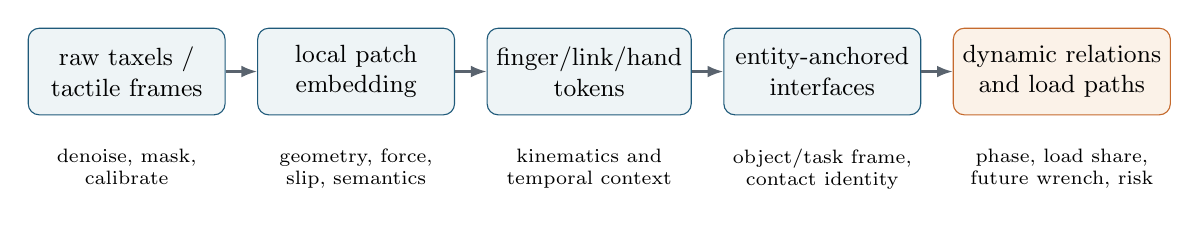
\begin{tikzpicture}[
  level/.style={draw=reviewblue, rounded corners, fill=reviewlight,
                minimum height=11mm, align=center, font=\small},
  goal/.style={draw=revieworange, rounded corners, fill=reviewwarm,
               minimum height=11mm, align=center, font=\small},
  arr/.style={-{Latex[length=2mm]}, thick, draw=reviewgray},
  node distance=4mm
]
\node[level, minimum width=25mm] (raw) {raw taxels /\\tactile frames};
\node[level, minimum width=25mm, right=of raw] (local) {local patch\\embedding};
\node[level, minimum width=25mm, right=of local] (body) {finger/link/hand\\tokens};
\node[level, minimum width=25mm, right=of body] (entity) {entity-anchored\\interfaces};
\node[goal, minimum width=27mm, right=of entity] (relation) {dynamic relations\\and load paths};
\draw[arr] (raw)--(local);
\draw[arr] (local)--(body);
\draw[arr] (body)--(entity);
\draw[arr] (entity)--(relation);

\node[font=\scriptsize, align=center, below=3mm of raw] {denoise, mask,\\calibrate};
\node[font=\scriptsize, align=center, below=3mm of local] {geometry, force,\\slip, semantics};
\node[font=\scriptsize, align=center, below=3mm of body] {kinematics and\\temporal context};
\node[font=\scriptsize, align=center, below=3mm of entity] {object/task frame,\\contact identity};
\node[font=\scriptsize, align=center, below=3mm of relation] {phase, load share,\\future wrench, risk};
\end{tikzpicture}
\caption{Representation hierarchy. The arrows denote additional organization,
not a mandatory neural architecture. Cross-interface claims require evidence at
the rightmost levels, even when the local encoder is strong.}
\label{fig:representation_hierarchy}
\end{figure}

\subsection{Local self-supervised and transferable touch}

Self-supervised tactile learning replaces expensive per-task labels with
objectives such as reconstruction, masked prediction, temporal consistency, and
instance discrimination. T-Dex couples pretraining to robotic play, showing that
unlabeled interaction can benefit downstream dexterity~\cite{guzey2023tdex}.
Sparsh scales self-supervision over vision-based tactile data and evaluates a
family of downstream tasks~\cite{higuera2025sparsh}. These approaches establish
that generic visual backbones are not enough and that tactile-specific pretraining
can be reused.

Transfer across sensors is harder because pixels encode different elastomers,
illumination, marker patterns, optics, and spatial scales. UniTouch learns unified
multimodal tactile representations~\cite{yang2024unitouch}; AnyTouch explicitly
addresses static and dynamic information across multiple visuo-tactile sensors
~\cite{feng2025anytouch}; T3 studies transferable Transformers
~\cite{zhao2024t3}; and UniT uses a unified tactile modelling approach
~\cite{xu2024unit}. Sparsh-X broadens the multisensory alignment setting
~\cite{higuera2025sparshx}, while TactAlign maps human tactile-glove features into
a robot tactile space for cross-embodiment transfer~\cite{tactalign2026}. The
common scientific question is not simply whether
embeddings transfer, but which tactile factors remain identifiable after
alignment. A sensor-invariant latent that collapses shear direction or scale may
be detrimental to load-path reasoning.

Whole-hand and morphology-aware models extend the unit of representation. HTT
uses heterogeneous tactile tokenization and masked learning~\cite{bi2026htt};
FTP-1 incorporates sensor morphology in a large tactile policy
~\cite{yuan2026ftp1}; HT-Bench supplies a whole-hand benchmark with egocentric
vision~\cite{huang2026htbench}. These works motivate explicit metadata for sensor
location, normal direction, link identity, and quality. In bimanual systems,
morphology-awareness must also prevent a shortcut in which ``left'' and ``right''
sensor IDs stand in for task role.

\subsection{Temporal tactile representations}

Touch is an event stream. Static contact appearance can be ambiguous: the same
deformation may correspond to loading or unloading, stable stick or the moment
before slip, depending on recent history. TactileVAD highlights geometric
aliasing in learned tactile dynamics~\cite{oller2023tactilevad}. Reactive control
systems increasingly split slow semantic reasoning from fast tactile reaction;
T-Rex uses tactile-reactive control at different time scales~\cite{niu2026trex},
while recent slow--fast visuo-tactile diffusion policies pursue a related control
principle. ViTacFormer also includes future-touch prediction as part of
cross-modal representation learning~\cite{heng2025vitacformer}.

Temporal modelling choices include fixed windows, recurrent states, temporal
convolution, causal Transformers, and state-space models. Their comparison is
often confounded by receptive field, parameter count, and action history. For
contact-transition evaluation, causal alignment is essential: a future tactile
frame may be a valid training target, but it must not leak into the deployed
encoder input. Reporting should distinguish synchronous state estimation,
$100$--$300$ ms forecasting, and closed-loop reaction.

\subsection{Multimodal fusion and spatial anchoring}

Tactile measurements acquire meaning from proprioception and vision. Early or
late concatenation is a strong baseline because a sufficiently expressive
temporal model can learn cross-modal interactions. Cross-attention gives tactile
tokens selective access to image, state, or action tokens; ViTacFormer is a
prominent recent example~\cite{heng2025vitacformer}. The fair question is whether
a proposed structure improves over this baseline at equal observation, compute,
and temporal context.

Spatial anchoring transforms local touch into a shared frame. SaTA anchors tactile
awareness using forward kinematics, enabling spatial reasoning beyond sensor
index~\cite{huang2025sata}. Object-centric approaches similarly normalize motion
with respect to the manipulated entity~\cite{chen2024objectcentric}. Anchoring is
particularly valuable for two hands because corresponding tactile features lie
in separate kinematic trees. Yet anchoring assumes that the relevant transform is
known or perceived; errors in link calibration and object pose should be tested,
not hidden.

\subsection{What existing objectives supervise}

\begin{table}[t]
\centering
\caption{Representation families, what they organize, and the unresolved
cross-interface question. Entries are representative rather than exhaustive.}
\label{tab:representation_families}
\begin{tabularx}{\linewidth}{P{0.18\linewidth} P{0.23\linewidth} P{0.25\linewidth} Y}
\toprule
\textbf{Family} & \textbf{Representative works} & \textbf{Primary organization} & \textbf{Unresolved bimanual question} \\
\midrule
Local SSL & T-Dex, Sparsh~\cite{guzey2023tdex,higuera2025sparsh} & contact appearance, geometry, dynamics & Does the latent retain load magnitude/direction and interface identity? \\
Cross-sensor alignment & UniTouch, AnyTouch, T3, Sparsh-X, TactAlign~\cite{yang2024unitouch,feng2025anytouch,zhao2024t3,higuera2025sparshx,tactalign2026} & shared tactile factors across hardware & Which physically relevant factors are lost to invariance? \\
Whole-hand / morphology-aware & HTT, HT-Bench, FTP-1~\cite{bi2026htt,huang2026htbench,yuan2026ftp1} & sensor layout, link/body coverage & Can roles and topology transfer across two heterogeneous hands? \\
Temporal dynamics & TactileVAD, T-Rex~\cite{oller2023tactilevad,niu2026trex} & event history and action-conditioned change & Are contact transitions predicted causally, before control action? \\
Cross-modal attention & ViTacFormer~\cite{heng2025vitacformer} & vision--touch--state token interaction & Does explicit interface structure add value to matched attention? \\
Spatial anchoring & SaTA~\cite{huang2025sata} & tactile features in kinematic space & How robust is the representation to pose error and topology change? \\
\bottomrule
\end{tabularx}
\end{table}

Pretraining objectives privilege different information. Reconstruction preserves
pixel detail but may waste capacity on illumination or marker appearance. Masked
prediction encourages context use but can exploit spatial redundancy. Contrastive
alignment emphasizes shared content but can suppress modality-specific physical
signals. Future prediction encodes dynamics but may average multimodal outcomes.
Task reward discovers control-relevant features but can exploit spurious state or
demonstration regularities. No objective is universally correct; its sufficiency
must be judged against the intended quantities and topology.

For bimanual coordination, promising auxiliary targets include contact onset and
release, future interface occupancy, load-share ratio, future local wrench, slip
risk, and calibrated uncertainty. These are not merely extra labels. They test
whether the latent exposes a mechanism that a downstream policy could use. Where
labels are available only in simulation, privileged-to-observation distillation
can train an observable student, but evaluation must verify that the student does
not require privileged inputs at test time.

\subsection{Necessary baselines for representation claims}

A new structured encoder should be compared against more than raw concatenation.
At minimum, a matched study should include: proprioception-only; tactile-only;
concatenation with the same local encoder; cross-attention; a temporal Transformer
or recurrent model; spatial anchoring where poses are available; a static graph;
the proposed inferred structure; and an oracle structure used only as an upper
bound. Parameter count, input history, optimization budget, augmentations, and
pretraining data must be controlled or reported. Without these controls, an
improvement may come from capacity, temporal context, or privileged supervision
rather than representation structure.

\section{Graphs, Contact Fields, and Physical Grounding}
\label{sec:structured}

\subsection{A graph is a hypothesis about factorization}

Interaction Networks established a general relational inductive bias: entities
and their pairwise relations can be modelled separately, with messages aggregated
to update entity states~\cite{battaglia2016interaction}. NerveNet applies graph
policies over articulated morphology~\cite{wang2018nervenet}; graph simulators
learn physical dynamics over interacting particles or bodies
~\cite{sanchez2020gns}; Graphormer demonstrates that Transformer attention can be
modified with graph-structural encodings~\cite{ying2021graphormer}; and AnyMorph
studies policies across morphologies~\cite{trabucco2022anymorph}. Together these
works make ``uses a GNN'' an architectural choice, not a sufficient novelty claim.

For tactile bimanual manipulation, a graph encodes a stronger hypothesis: task
dynamics factorize around interfaces and the paths connecting them. This
hypothesis is useful only if (i) node and edge semantics correspond to deployable
or inferable quantities, (ii) the factorization improves sample efficiency,
robustness, interpretability, or intervention response, and (iii) the same gain
cannot be explained by additional state or parameters.

\subsection{Taxel, finger, and morphology graphs}

Graph construction at the tactile-array or finger level is relatively direct.
Distributed tactile sensors have known positions on an articulated hand;
convolution or message passing can share information along this geometry.
Multi-finger in-hand manipulation with distributed tactile GCNs demonstrates this
idea~\cite{funabashi2022distributed}. TacGNN uses hierarchical graph structure for
blind tactile-based in-hand manipulation~\cite{yang2023tacgnn}. TactiGraph treats
event-based tactile measurements asynchronously for contact-angle prediction
~\cite{sajwani2023tactigraph}, and TouchWGNN develops spatio-temporal tactile
graphs for multimodal dexterous manipulation~\cite{ning2026touchwgnn}.

These models address meaningful spatial and temporal organization. However, a
taxel adjacency graph is not the same as a dynamic task contact graph. Taxels can
remain neighbours in the sensor layout whether or not their links contact the
same object; fingers can be kinematically adjacent while transmitting loads
through different entities. Bimanual load-path work therefore needs at least two
levels: relatively stable morphology/sensor structure and dynamic inter-entity
interfaces.

\subsection{Dynamics graphs and contact discontinuities}

RoboPack learns tactile-informed recurrent graph dynamics for dense packing and
uses the model for planning/control~\cite{ai2024robopack}. Its relational
factorization is compelling because tool, objects, and environment interact over
time. ContactNets targets discontinuous contact dynamics with a structured
implicit model~\cite{pfrommer2020contactnets}; graph network simulators have been
shown to model rigid contact transitions~\cite{allen2022contact}. This line of
work suggests two design principles for bimanual representation: predict changes
at interfaces, and avoid treating discontinuity as ordinary smooth motion noise.

MeshPriorDiT adds a useful hierarchical counterexample to an architecture-only
comparison. An action-conditioned mesh GNN supplies topology and grasp-constraint
priors, while a flow-matching diffusion Transformer models residual and global
cloth effects~\cite{wang2026meshpriordit}. Its evidence concerns deformable mesh
dynamics rather than tactile load transfer, but the factorization is directly
relevant: structured local priors and expressive global residuals can be
complementary. A bimanual study should therefore compare graph-only,
global-residual-only, and combined models rather than forcing a false GNN-versus-
Transformer dichotomy.

Yet dynamics prediction can be correct for the wrong reason. Exact object pose,
collision geometry, and contact labels can make a simulator graph accurate while
an observation-only system remains underdetermined. A useful paper must specify
which signals construct the graph at training and at deployment. ``Physics
grounded'' should describe targets, conservation constraints, frames, or
interventions---not merely that the task occurs in a physics engine.

Dex-X makes the distinction between removing privileged state and removing
reference dependence concrete~\cite{chen2026dexx}. Its spatialized tactile-force
student drops current object-pose and geometric privileged blocks but retains
next-step motion references and the demonstration's target object pose. Its
bimanual handover result belongs to simulation; real evaluation includes
single-hand manipulation with strongly mixed object-generalization outcomes.
This is a useful spatialized-force and distillation comparator, but should not be
called reference-free, real bimanual load-path inference, or topology transfer.
CoRL acceptance was author-reported at this audit, not independently confirmed
from an official venue record.

\subsection{Contact fields, modes, and anchors}

Graphs are not the only structured representation. Neural Contact Fields track
extrinsic contact through tactile sensing~\cite{higuera2023ncf}; object-centric
contact-field approaches extend this spatial view to visuo-tactile state
estimation and tool interaction. Semantic Contact Fields predict semantically
meaningful contact/force structure for tool manipulation
~\cite{ma2026semanticcontact}. Contact-mode control represents discrete
constraint regimes for non-prehensile manipulation~\cite{oller2024extrinsic}.
Contact-anchored policies and contact-grounded policy learning similarly use
contact as a privileged or learned organizing variable
~\cite{cui2026contactanchored,xu2026contactgrounded}.

Recent work also clarifies two meanings of ``contact structure.'' One-shot
learning by identifying physical interactions extracts making/breaking contact
events from a demonstration and uses them as transition conditions for hybrid
position--force control~\cite{overbeek2026oneshot}. CoToGrasp conditions grasp
synthesis on a requested contact topology in a canonical workspace
~\cite{merand2026cotograsp}. Both make structure explicit, but the former uses a
demonstrated event state machine and the latter a prescribed grasp-contact layout.
Neither is equivalent to inferring a time-varying cross-hand topology from raw
deployment observations. They are valuable controls precisely because they test
how much structure can be specified rather than learned.

CADeT is positive evidence that useful interaction structure need not be supplied
as simulator truth~\cite{hu2026cadet}. It infers a belief over predefined coupled,
decoupled, and blocked tissue-transmission modes from visually tracked responses
and physical probes. In 150 simulation trials with mode truth withheld, it
identifies 149 modes correctly; matched information-guided probes require fewer
additional actions than random probes. Phantom and ex-vivo experiments extend
the evidence beyond simulation. This is visual, fixed-family mode inference,
with nominal calibration before blockage, rather than tactile cross-hand graph
inference or held-out-participant topology transfer. GP covariance informs mode
likelihoods but is not propagated through the MPC horizon; entropy convergence
is not probability-calibration evidence, and contact force/strain safety is not
measured or guaranteed.

Fields are attractive when contact location varies continuously over object
surfaces; discrete graphs are attractive when entity/interface identity and
message routing matter. Hybrid representations can use a field to infer contact
location and confidence, then instantiate an entity-level relation. The decisive
comparison should be empirical: a field, graph, anchored token set, and
unstructured attention model should receive the same observations and predictive
targets.

\begin{table}[t]
\centering
\caption{Structured-representation choices. The final column states what must be
demonstrated rather than assumed.}
\label{tab:structured_models}
\begin{tabularx}{\linewidth}{P{0.18\linewidth} P{0.21\linewidth} P{0.25\linewidth} Y}
\toprule
\textbf{Structure} & \textbf{Natural unit} & \textbf{Typical source} & \textbf{Validity test} \\
\midrule
Sensor/morphology graph & taxel, link, joint & calibrated layout and kinematics & robustness across layouts, missing sensors, and embodiments \\
Static task graph & hand, object, tool & designer-specified entity relations & advantage over matched attention without dynamic edge changes \\
Dynamic contact graph & active interface & tactile/proprioceptive inference or simulator contact & inferred--oracle gap, transition timing, false-edge interventions \\
Object-centric anchor & local feature in object frame & visual/kinematic pose estimate & degradation under pose error and unseen grasps \\
Contact field & continuous surface point/force & tactile/vision and geometry & contact localization, force consistency, surface/OOD generalization \\
Contact mode & discrete constraint regime & estimator, demonstration, or privileged label & mode-transition accuracy and closed-loop recovery \\
Physics residual/constraint & force balance, momentum, complementarity & measured or simulated quantities & calibration, counterfactual consistency, no label circularity \\
\bottomrule
\end{tabularx}
\end{table}

\subsection{PhysGraph as a boundary case}

PhysGraph is a directly relevant early graph-policy formulation for bimanual
hand--tool--object manipulation~\cite{li2026physgraph}. It organizes hand, tool,
and object information in a graph Transformer and reports strong simulated
control. Its input regime, however, includes simulator state, fingertip resultant
forces, object/tool geometric encodings, and future reference. It should therefore
be read as evidence for relational policy factorization under privileged state,
not as tactile-array representation pretraining or observation-grounded contact
inference.

A local audit of the public main-branch snapshot at the corpus freeze found that
the bias generator exposes contact-mask and geometric-position inputs, while the
default forward call does not pass them; the resulting public path uses the
configured topology rather than the advertised dynamic contact/geometric bias.
This is a reproducibility observation about that code snapshot, not evidence that
the authors' reported experiments used the same path. The correct experimental
response is to reproduce both the stock public path and a clearly documented
corrected-bias path, then avoid attributing their difference to the paper without
author confirmation.

This case illustrates why code-level observability matters. A diagram can show
dynamic edges while the executed model uses static connectivity; a paper can
describe tactile feedback while the input is a low-dimensional simulator force;
and a physically plausible target can be constructed from unavailable future
state. Reproduction should trace every tensor from sensor or simulator source to
the model and record its deployment availability.

\subsection{Physical objectives for cross-interface structure}

Suppose an inferred interface edge $e_{ij,t}$ has probability $p_{ij,t}$ and an
estimated wrench $\hat{\bm w}_{ij,t}$ expressed in a common object frame. Useful
objectives can combine:

\begin{equation}
\mathcal{L} = \lambda_e \mathcal{L}_{\text{edge}}
 + \lambda_w \mathcal{L}_{\text{future-wrench}}
 + \lambda_s \mathcal{L}_{\text{slip}}
 + \lambda_p \mathcal{L}_{\text{phase}}
 + \lambda_c \mathcal{L}_{\text{consistency}}.
\label{eq:physical_loss}
\end{equation}

The consistency term might penalize disagreement between predicted interface
wrenches and measured object acceleration or enforce action--reaction relations
when both sides of an interface are observed. It should be soft and
uncertainty-aware: unmodelled compliance, gravity-compensation error, and
unobserved environmental contact make exact balance inappropriate. The model
should also predict confidence, because a missing edge under sensor occlusion is
not equivalent to a confidently absent contact.

For sustained contact, the state should additionally represent slow relaxation.
Temperature-coupled viscoelastic force estimation shows that identical-looking
instantaneous configurations can correspond to different force histories
~\cite{wang2026relaxation}. Interface objectives should therefore be evaluated at
multiple contact durations and, where relevant, condition on temperature or an
identified relaxation state rather than treating drift as independent noise.

The central empirical question remains comparative. If a temporal Transformer
with the same inputs predicts future wrench and phase equally well, explicit
edges may add interpretability but not predictive value. If structure improves
data efficiency, transition accuracy, or transfer to a new topology---and the
benefit disappears under random or time-shuffled edges---the relational
hypothesis receives stronger support.

\section{Bimanual Coordination, Handover, and Cooperative Tool Use}
\label{sec:bimanual}

\subsection{Bimanual learning is broader than tactile coordination}

Bimanual manipulation has grown rapidly through simulation benchmarks,
retargeting, imitation, and scalable demonstration generation. Bi-DexHands
provides a broad simulated reinforcement-learning benchmark
~\cite{chen2022bidexhands}. Bimanual Dexterity for Complex Tasks and related real
systems demonstrate increasingly capable coordinated policies
~\cite{shaw2024bidex}. DexMimicGen generates bimanual data from demonstrations
~\cite{jiang2024dexmimicgen}; ManipTrans transfers behaviours through residual
learning~\cite{li2025maniptrans}; object-centric human-motion approaches organize
demonstrations around manipulated objects~\cite{chen2024objectcentric}. These
works establish task and data scalability. They do not automatically test whether
a tactile latent explains cross-hand forces or contact transitions.

Late-August work further raises the vision/proprioception-only baseline.
Training-time modality masking improves robustness of a query-based bimanual VLA
without adding a tactile relation model~\cite{cheng2026modalitymasking};
PartialBiGrasp infers hidden local geometry from partial point clouds and searches
for force-closure-compatible grasp pairs~\cite{kaura2026partialbigrasp}. CLAP
learns a cross-embodiment action-conditioned video world model with bimanual data
among its supported settings~\cite{liu2026clap}, while rapid on-robot juggling
learns local dynamic models around a global prior under a reachable safe-set
constraint~\cite{lee2026robotjuggling}. Together they explain more bimanual
success through visual geometry, robust fusion, video prediction, and rapid
dynamics adaptation. A tactile representation must therefore demonstrate an
incremental benefit under occlusion, friction change, slip, or simultaneous load
transfer, not rely on bimanual task success alone.

This distinction matters for literature positioning. The broad claim ``bimanual
manipulation is underexplored'' is no longer defensible. The narrower intersection
of \emph{observation-grounded tactile structure}, \emph{explicit interface/load
targets}, and \emph{matched representation comparisons} remains much less
populated in the mapped corpus. A contribution should therefore be framed around
that intersection, not around the existence of two hands.

Bi-Touch is an important early direct baseline: it used a concatenated tactile
policy state and sim-to-real reinforcement learning for contact-rich bimanual
pushing, reorientation, and gathering tasks~\cite{bitouch2023}. It shifted the question from whether
touch can help bimanual control to whether an explicit relational representation
adds value beyond a matched tactile policy input. A new graph method should
therefore include an equivalent concatenation baseline even if the original
Bi-Touch implementation is not the primary reproduction target.

\subsection{Roles, symmetry, and mechanical necessity}

A bimanual taxonomy can distinguish symmetric and asymmetric actions, shared and
separate objects, coordinated and independent motions, and temporal role changes
~\cite{krebs2022taxonomy}. For representation research, two additional questions
are decisive:

\begin{enumerate}
  \item \textbf{Is coordination mechanically necessary?} If one hand can complete
  the task while the other supplies a decorative or easily ignored motion, task
  success does not diagnose cross-hand representation.
  \item \textbf{Can the roles be exchanged?} A representation that encodes fixed
  left/right identities may fail when actor and stabilizer swap, even though the
  physical relation is unchanged.
\end{enumerate}

BUDS makes stabilizer--actor coordination explicit and demonstrates that one hand
can create conditions for the other~\cite{grannen2023stabilize}. This is a useful
conceptual bridge from shared-object manipulation to tool--workpiece tasks.
However, role assignment should be coupled to measurable necessity: removing,
delaying, or perturbing the stabilizing hand ought to change forces, error, or
success in a predictable way.

\subsection{Handover as a load-transfer benchmark}

Handover provides an unusually clean phase structure. Human-inspired and
robot--robot/robot--human controllers have long used load, pull, grip force, or
slip cues to govern transfer and release~\cite{costanzo2021handover}. Contact-aware
dexterous handover further emphasizes when and where contacts occur
~\cite{wang2024contacthandover}. VTDexManip supplies a reproducible simulated
bimanual handover task with visual-tactile observations
~\cite{liu2025vtdexmanip}; recent tactile-reactive systems expand the scale and
realism of bimanual touch~\cite{niu2026trex}.

The most informative handover interval is dual contact. Let $F_L(t)$ and $F_R(t)$
be gravity-axis support estimates expressed in a common object frame. A simple
load-share target is

\begin{equation}
\rho_R(t)=\frac{\max(0,F_R(t))}
{\max(0,F_L(t))+\max(0,F_R(t))+\epsilon}.
\label{eq:loadshare}
\end{equation}

This ratio is interpretable and less scale-sensitive than absolute force, but it
is only valid if the force estimates are independently calibrated and frame
aligned. Contact phase, time-to-support, future receiver wrench, giver slip risk,
and release readiness provide complementary targets. The point is not to impose
one scalar definition; it is to make the transfer mechanism measurable.

Dynamic throw--catch handover explores timing, ballistic motion, and impact
recovery~\cite{huang2023dynamichandover}. It should be a later robustness task
rather than the primary cross-hand load benchmark, because the flight phase
removes the simultaneous object-mediated path. A quasi-static transfer with a
speed perturbation, object-mass change, or receiver delay offers cleaner causal
tests first.

Robot juggling reinforces this sequencing: impressive rapid online adaptation in
a dynamic bimanual task can be achieved from onboard vision and a local dynamics
model~\cite{lee2026robotjuggling}. It is therefore a strong adaptation reference,
but its flight/contact alternation does not provide the persistent, simultaneous
object-mediated load path needed to validate cross-hand tactile structure.

\subsection{Cooperative tool--workpiece manipulation}

One hand holding a brush while the other holds a plate is closely aligned with the
same representation problem, but its topology is more demanding. The actor hand
senses its grasp on the tool; the stabilizer hand senses the workpiece; the
working interface between brush and plate is remote from both local grasp
interfaces. Force and motion propagate through at least three contacts. This task
therefore tests whether a representation can move from
$H_L\!\leftrightarrow O\!\leftrightarrow H_R$ to
$H_L\!\leftrightarrow T\!\leftrightarrow W\!\leftrightarrow H_R$.

The adjacent literature supplies components rather than a saturated direct
benchmark. Tactile Tool Manipulation learns tool-related control with tactile
feedback~\cite{shirai2023tactiletool}; compliant tool--environment dynamics and
extrinsic contact-mode control model the working interface
~\cite{vandermerwe2022compliant,oller2024extrinsic}; RoboPack demonstrates
tactile-informed relational dynamics in tool-mediated dense contact
~\cite{ai2024robopack}; TACO covers tool--action--object semantics
~\cite{liu2024taco}; TAMEn targets tactile-aware closed-loop data collection in
contact-rich tasks such as dish washing~\cite{wu2026tamen}; and Semantic Contact
Fields make tool contacts explicit~\cite{ma2026semanticcontact}. These works make
the area adjacent, not empty. What remains scarce is a controlled study of
\emph{cross-hand tactile load propagation} with a held workpiece and matched
representation baselines. TAMEn is a direct system competitor for a dish-washing
demonstration; novelty cannot rest on performing that task with touch, but must
come from observation-grounded load-path inference, mechanism-level evidence, or
cross-topology transfer.

\begin{table}[t]
\centering
\caption{How the two principal task families complement each other. ``Mapped
evidence density'' is a qualitative inference from the curated corpus, not a
bibliometric claim.}
\label{tab:handover_tool}
\begin{tabularx}{\linewidth}{P{0.19\linewidth} Y Y}
\toprule
 & \textbf{Quasi-static handover} & \textbf{Cooperative tool--workpiece use} \\
\midrule
Core topology & hand--object--hand, changing support & hand--tool--workpiece--hand, persistent role asymmetry \\
Primary signal & load redistribution and release & working-contact wrench, stabilizer reaction, slip \\
Main advantage & clean phases and interpretable transition & harder multi-hop transfer and practical task relevance \\
Main confound & object pose/motion can reveal phase & visual trajectory, periodic motion, and compliance can reveal task state \\
Mapped evidence density & established handover/control literature; few matched representation studies & established tool/contact systems; few matched cross-hand load-flow studies \\
Best research role & first controlled representation benchmark & gated second topology after mechanism is established \\
\bottomrule
\end{tabularx}
\end{table}

\subsection{Designing a diagnostic tool task}

A diagnostic task should make the second hand necessary while remaining simple
enough to label. A rigid stylus or wiping puck against a plate is preferable to a
deformable brush for an initial experiment: the contact location, normal, and
applied path can be controlled, and simulation is more credible. The task can
then progress to a compliant brush once sensing and analysis are stable.

Useful experimental factors include tool stiffness, workpiece mass, friction,
path curvature, contact-force target, stabilizer grasp, actor/stabilizer role
swap, and brief perturbations of either hand. A \emph{coordination-necessity
check} should compare two hands, fixed workpiece, passive second hand, and removed
second-hand tactile input. If the actor succeeds with no measurable cost when the
stabilizer is removed or frozen, the task is not a strong cross-hand benchmark.

The tool task should enter a research programme after the simpler handover study
has established three points: inferred structure improves at least one
transition/load target over matched unstructured baselines; the gain is not due
to privileged state; and structure remains useful under object/grasp holds-out.
Before those conditions, tool use is valuable as a frozen task specification and
offline proxy, but a full hardware campaign risks combining unsolved sensing,
calibration, control, and representation problems.

\subsection{Cross-topology transfer as the stronger claim}

Training and testing separately on handover and tool use would produce two task
results. A stronger representation claim asks whether a model pretrained to infer
interfaces and loads on handover transfers to the longer tool topology with
fewer labels or demonstrations. The test should distinguish:

\begin{itemize}
  \item \textbf{encoder transfer:} freeze the local tactile encoder and retrain
  only the relation head;
  \item \textbf{relation transfer:} preserve edge functions while instantiating a
  new entity topology;
  \item \textbf{full fine-tuning:} initialize all weights and measure data
  efficiency;
  \item \textbf{zero-shot probing:} test whether phase/load variables are linearly
  recoverable without task fine-tuning.
\end{itemize}

If only full fine-tuning helps, the model may provide generic initialization rather
than compositional topology transfer. If relation modules transfer under role
swap and added tool/workpiece nodes, the evidence for structured factorization is
substantially stronger.

\section{Evaluation: From Task Success to Representation Evidence}
\label{sec:evaluation}

\subsection{Why task success is insufficient}

Closed-loop success is necessary for a control method but weak evidence about a
specific latent mechanism. A policy can infer phase from vision, memorize object
trajectories, exploit a scripted receiver, or rely on privileged object state.
It may succeed without using tactile inputs at all. Conversely, a representation
can predict contact transitions accurately while a poorly tuned controller masks
the benefit. Evaluation should therefore connect four levels: observation
integrity, representation probes, open-loop dynamics, and closed-loop behaviour.

\begin{figure}[t]
\centering
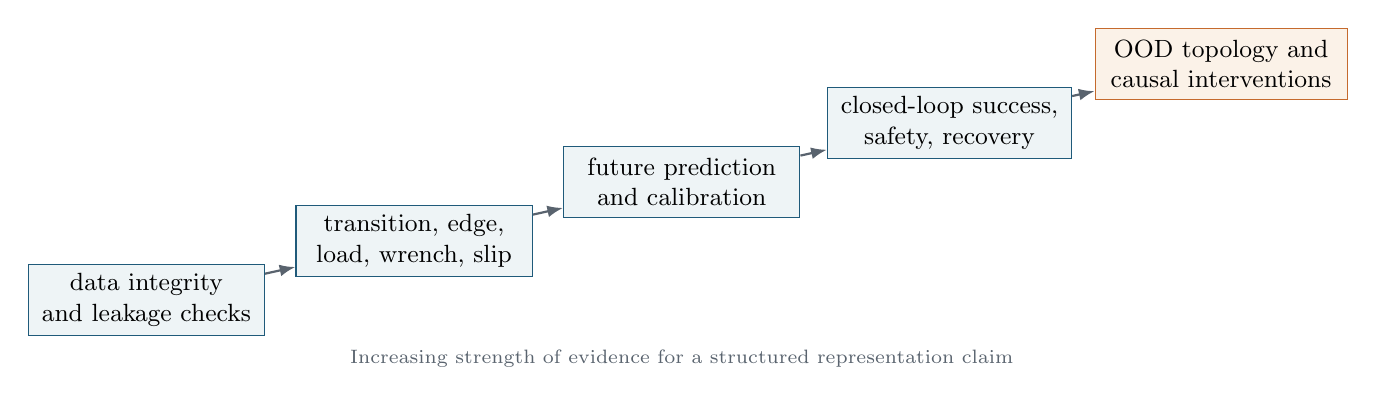
\begin{tikzpicture}[
  rung/.style={draw=reviewblue, fill=reviewlight, minimum height=9mm,
               align=center, font=\small},
  strong/.style={draw=revieworange, fill=reviewwarm, minimum height=9mm,
                 align=center, font=\small},
  arr/.style={-{Latex[length=2mm]}, thick, draw=reviewgray}
]
\node[rung, minimum width=30mm] (integrity) at (0,0) {data integrity\\and leakage checks};
\node[rung, minimum width=30mm] (probe) at (3.4,0.75) {transition, edge,\\load, wrench, slip};
\node[rung, minimum width=30mm] (pred) at (6.8,1.5) {future prediction\\and calibration};
\node[rung, minimum width=31mm] (control) at (10.2,2.25) {closed-loop success,\\safety, recovery};
\node[strong, minimum width=32mm] (causal) at (13.65,3.0) {OOD topology and\\causal interventions};
\draw[arr] (integrity)--(probe);
\draw[arr] (probe)--(pred);
\draw[arr] (pred)--(control);
\draw[arr] (control)--(causal);
\node[font=\scriptsize, text=reviewgray] at (6.8,-0.75) {Increasing strength of evidence for a structured representation claim};
\end{tikzpicture}
\caption{An evidence ladder for representation research. Higher rungs depend on,
rather than replace, the lower-level checks.}
\label{fig:evidence_ladder}
\end{figure}

\subsection{Matched-budget baseline matrix}

The baseline matrix in \cref{tab:baseline_matrix} isolates the source of an
improvement. All learned variants should share the same local tactile encoder,
observations, history, training examples, optimizer budget, and approximately
matched parameter/compute count. If a graph variant receives link poses while a
Transformer does not, the study tests information access, not factorization.
Two additional controls are necessary after the core-paper audit. A predictive
contact-grounding baseline tests whether future tactile/state objectives alone
explain the gain~\cite{heng2025vitacformer,xu2026contactgrounded}; a dynamic taxel
graph tests whether local sensor-level message passing already suffices
~\cite{ning2026touchwgnn}.
The surveillance update adds three more controls: a directed contact--deformation--
slip predictor~\cite{xue2026hitacwam}, training-only temporal-flow grounding
~\cite{yang2026temporalflowvla}, and prediction-error recurrent inference
~\cite{sawada2026predvla}. Cross-embodiment visual prediction such as CLAP is a
useful system-level baseline where video pretraining is available
~\cite{liu2026clap}, but it must receive the same deployment observations when
used to isolate the value of touch.

\begin{table}[t]
\centering
\caption{Minimum matched-budget experiment matrix. The oracle graph is an upper
bound and must never be presented as a deployable method.}
\label{tab:baseline_matrix}
\begin{tabularx}{\linewidth}{P{0.20\linewidth} C C C Y}
\toprule
\textbf{Model} & \textbf{Same local encoder} & \textbf{Temporal context} & \textbf{Explicit structure} & \textbf{Question isolated} \\
\midrule
Proprioception-only & n/a & matched & none & Is touch needed? \\
Tactile concat & \yes & matched & none & Does local touch help? \\
Cross-attention & \yes & matched & implicit & Is flexible token interaction sufficient? \\
Temporal Transformer & \yes & matched & implicit & Is time/context the main source of gain? \\
Prediction-error recurrent & \yes & matched & implicit/predictive & Does observation-driven latent correction explain the gain? \\
Predictive grounding & \yes & matched & implicit/predictive & Do future tactile/state objectives explain the gain? \\
Directed tactile hierarchy & \yes & matched & ordered physical heads & Does contact $\rightarrow$ deformation $\rightarrow$ slip ordering beat flat heads? \\
Training-only temporal grounding & \yes & matched & privileged supervision only & Does richer training supervision, rather than deployed structure, explain the gain? \\
Spatially anchored tokens & \yes & matched & coordinates & Does a shared frame suffice? \\
Dynamic taxel graph & \yes & matched & local learned edges & Does sensor-level graph structure suffice? \\
Static graph & \yes & matched & fixed edges & Does relational routing help without edge inference? \\
Inferred dynamic graph & \yes & matched & observed/inferred & Does topology inference add value? \\
Oracle graph & \yes & matched & privileged edges & What is the attainable structural upper bound? \\
Random / shuffled graph & \yes & matched & invalid control & Does edge semantics, rather than regularization, matter? \\
\bottomrule
\end{tabularx}
\end{table}

\FloatBarrier

For the tool-use phase, contact-centric alternatives are also mandatory: compare
system-level interface edges with a continuous contact-field condition and a
contact-anchored policy frame~\cite{ma2026semanticcontact,cui2026contactanchored}.
These are phase-specific baselines rather than reasons to give the graph model
extra geometry or labels.

A useful diagnostic is the fraction of oracle improvement retained by inferred
structure. Let $M$ be a higher-is-better metric and $M_U$, $M_I$, and $M_O$ the
unstructured, inferred, and oracle scores. Then

\begin{equation}
R_{\mathrm{oracle}}=
\frac{M_I-M_U}{M_O-M_U+\epsilon}.
\label{eq:oracle_retention}
\end{equation}

This ratio is descriptive, not a universal target. It is unstable when the oracle
gain is small and should always be reported with raw scores and uncertainty. For
error metrics, the signs must be adjusted. Its value is that it distinguishes a
weak edge estimator from an unhelpful structural hypothesis.

\subsection{Metrics aligned to the claimed mechanism}

\paragraph{Contact and phase.}
Use per-class precision, recall, and macro-F1 for giver-only, dual-contact,
receiver-only, no-contact, tool-contact, and slip states. Frame accuracy should be
supplemented with transition timing error, segment-level F1, and early-warning
horizon. Long stable segments otherwise dominate the score.

\paragraph{Edges.}
Dynamic-edge evaluation requires precision--recall AUC under class imbalance,
onset/offset timing, false persistent edges, and calibration. Node/edge identity
must be permutation-consistent where appropriate. Testing only edges used to
construct training labels risks circularity; held-out contact configurations and
sensor ablations are stronger.

\paragraph{Load and wrench.}
Report load-share MAE, absolute force/wrench MAE in a stated frame, angular error
for force direction, normalized error across object masses, and horizon-specific
future prediction. Estimated tactile wrench should not be described as independent
ground truth. Gravity compensation, filtering, and coordinate transformations
belong in the method, not supplementary guesswork.

\paragraph{Slip and uncertainty.}
Slip is an event-detection problem with severe imbalance. Precision--recall,
false alarms per minute, and warning time are more informative than accuracy.
Fine-grained contact-state and slip-direction sensing provides a concrete local
classification reference~\cite{ma2026slip}, but local class accuracy should not
be reported as evidence of cross-interface load inference.
For uncertainty, use reliability diagrams, expected calibration error, Brier
score, negative log likelihood, and risk--coverage curves. Calibration should be
re-evaluated under object, sensor, and topology shift.

\paragraph{Duration, relaxation, and damage.}
Sustained-contact evaluation should stratify error by contact duration,
temperature, material, and load/unload history; relaxation-aware force sensing
shows why a single aggregate MAE can hide systematic drift
~\cite{wang2026relaxation}. For deformable objects, report task success and a
separate deformation or damage constraint. SoftVTBench's deformation-aware
success rate is one example of requiring both completion and bounded peak
deformation~\cite{jing2026softvtbench}; the exact threshold and evaluator-only
state must remain explicit.

\paragraph{Closed-loop outcomes.}
Success should be paired with time, peak force, impulse, drop rate, object damage
proxy, path error, number of recovery events, and unnecessary grip. A structured
model that achieves the same success with lower peak force or earlier safe release
can still be valuable.
Failure-aware execution further requires separate accounting for detection,
local retry, reset/recovery, and irrecoverable failure. FLARE operationalizes
these branches with an online monitor and distinct retry/reset mechanisms
~\cite{zhao2026flare}; it is a visual--language recovery framework rather than a
tactile representation, but it makes recovery-aware metrics a necessary control
for long-horizon claims.

\subsection{Splits and out-of-distribution tests}

Random frame splits are invalid for temporally correlated episodes. The split
hierarchy should include, where relevant:

\begin{itemize}
  \item episode and contiguous contact-sequence holds-out;
  \item object identity, geometry, mass, friction, and compliance holds-out;
  \item grasp pose and hand-role swap;
  \item collection session, operator/demonstrator, and calibration session;
  \item sensor instance, sensor type, missing channels, and added latency;
  \item embodiment or morphology;
  \item task/contact topology, such as handover training and tool-use testing.
\end{itemize}

The split must be made before window extraction so adjacent windows cannot cross
train/test boundaries. Hyperparameter selection should use a validation split
with the same unit as the intended generalization claim.

The 30-paper full-text core contained zero studies that met a strict
contact-topology OOD criterion under deployment-observable inference. Strict
topology OOD holds out the contact-participant or edge structure itself (for
example, hand--object--hand training followed by hand--tool--workpiece--hand
testing). Unseen object instances, new tool geometry, contact-mode variation
within a fixed participant structure, and semantic tool--action composition are
valuable tests, but they must be reported separately rather than relabelled as
topology transfer.

\subsection{Causal and counterfactual interventions}

Correlational probes show what can be decoded; interventions show whether the
claimed structure matters. Low-cost interventions include time-shuffling one
hand's tactile stream, swapping left/right roles, masking one fingertip, delaying
receiver contact, perturbing the workpiece, rewiring predicted edges, or freezing
edge probabilities. Physical interventions include known mass/friction changes,
brief stabilizer motion, tool stiffness changes, or an unexpected contact. The
expected direction of change should be stated before the experiment.

For temporal baselines, mask history content, shuffle its order, and disable
observation-driven latent correction exactly rather than replacing the model with
an unrelated architecture. TemporalFlow-VLA and PredVLA make these interventions
especially concrete~\cite{yang2026temporalflowvla,sawada2026predvla}. For
hierarchical tactile prediction, compare flat heads, stop-gradient removal, and
dependency-order shuffling~\cite{xue2026hitacwam}.

For example, delaying receiver contact should delay load-share crossover and safe
release. If a model's phase prediction is unchanged, it may be following a motion
schedule rather than tactile evidence. Rewiring a tool--workpiece edge should
damage future-wrench prediction more than rewiring an inactive relation. If all
rewirings have equal effect, the graph may act as generic regularization.

\subsection{Statistics and reproducibility}

Formal results should use at least five independently seeded runs where training
variance is material; early internal decisions can use three seeds but must not be
reported as definitive. Pair results by the same data split and environment seed.
Report effect sizes and confidence intervals, not only significance tests. For
episode success, use bootstrap or binomial intervals with episode as the unit;
for dense time series, aggregate within episode before testing or use hierarchical
resampling.

Reproducibility requires a data lineage from raw sensor packet to metric: hashes or
version identifiers, synchronization configuration, calibration, split manifests,
normalization fitted only on training data, model configuration, seeds, software
environment, checkpoint selection, and evaluation script. Code audits should
distinguish a paper's claims from what a public snapshot executes, as illustrated
by the PhysGraph case in \cref{sec:structured}.

\begin{table}[H]
\centering
\caption{Claim-to-evidence checklist. A paper need not include every row, but the
evidence should match its stated contribution.}
\label{tab:claim_evidence}
\begin{tabularx}{\linewidth}{P{0.25\linewidth} Y Y}
\toprule
\textbf{Claim} & \textbf{Minimum comparison} & \textbf{Stronger evidence} \\
\midrule
Touch is necessary & proprio/vision-only and tactile ablation & sensor masking and latency interventions \\
Explicit structure helps & matched attention/temporal/static graph & random-edge control and oracle--inferred analysis \\
Edges are observation-grounded & no test-time privileged inputs & pose/sensor corruption and edge calibration \\
Representation is physical & interface/load predictive targets & force-balance residuals and counterfactual response \\
Generalizes & object/session/contact-sequence split & sensor, embodiment, role, and topology holds-out \\
Improves control & multi-seed success and safety metrics & disturbance recovery and risk--coverage analysis \\
\bottomrule
\end{tabularx}
\end{table}

\FloatBarrier

\section{Synthesis and Research Agenda}
\label{sec:agenda}

\subsection{What the literature currently supports}

The mapped evidence supports six qualified conclusions.

First, tactile-specific pretraining is useful. Across robotic play,
self-supervision, multimodal alignment, and cross-sensor learning, tactile
representations outperform purely task-specific training in several downstream
settings~\cite{guzey2023tdex,higuera2025sparsh,yang2024unitouch,feng2025anytouch}.
This justifies reusing a strong local encoder rather than learning raw tactile
features from scratch for every bimanual experiment.

Second, spatial and relational inductive biases can be useful when the task has
known structure. Morphology graphs, tactile graphs, object-centric dynamics, and
contact fields have succeeded in in-hand manipulation, physics prediction,
packing, and contact tracking~\cite{funabashi2022distributed,yang2023tacgnn,ai2024robopack,higuera2023ncf}.
This establishes plausibility, not universal superiority over attention.

Third, bimanual dexterity has become an active, increasingly crowded research
area. Large simulation suites, demonstration-generation systems, retargeting, and
real policies now cover many complex tasks
~\cite{chen2022bidexhands,shaw2024bidex,jiang2024dexmimicgen,li2025maniptrans}.
Novelty must therefore be located in a specific mechanism or evaluation gap.

Fourth, contact-centric and tactile-reactive control is moving toward broader
embodiments, tools, and data scales~\cite{niu2026trex,yuan2026ftp1,ma2026semanticcontact,madan2026tactic,zhou2026touchworld}.
Because many examples are recent preprints or programme-listed works, they define
a competitive frontier more than a settled empirical consensus.

Fifth, the strongest competing explanations are increasingly structured even
when they are not tactile graphs. Directed tactile prediction
~\cite{xue2026hitacwam}, mesh-prior plus diffusion-residual dynamics
~\cite{wang2026meshpriordit}, temporal-flow supervision
~\cite{yang2026temporalflowvla}, prediction-error recurrence
~\cite{sawada2026predvla}, and failure-aware recovery
~\cite{zhao2026flare} each isolate a different source of performance. This makes
matched objective, history, and recovery controls part of the minimum evidence
for an explicit contact-structure claim.

Sixth, direct evidence now reaches beyond isolated local tactile features.
BiView-Touch supports useful cross-hand predictive dependence in human recordings;
causal force-history plus compliance supports real bimanual release/hold decisions;
and CADeT supports visually inferred transmission modes with active probing
~\cite{liang2026biviewtouch,marra2026temporaltactilehandover,hu2026cadet}.
These results narrow the gap. They do not jointly demonstrate independent robot
load-path validity, matched structural benefit, calibrated uncertainty, and
held-out contact-participant topology. Meanwhile, ContactWorld and the October
SimpleTouch/VISTA controls make representation, goal information, and feedback
frequency separate competing explanations
~\cite{zhang2026contactworld,yang2026simpletouch,wong2026vista}.

\subsection{What the literature does not yet establish}

The evidence does not yet establish that an inferred dynamic contact graph is
better than a matched temporal Transformer for bimanual load transfer. It does not
establish that local tactile foundation models preserve cross-interface wrench
information. It does not yet establish robust, uncertainty-tested recovery of robotic
load-path topology from deployable touch and proprioception across changed
participant structures. It also does not provide a
standard benchmark for transfer from handover to cooperative tool use.

These gaps are linked by an evidence chain:

\begin{equation}
\begin{aligned}
\text{sensor signal} &\rightarrow \text{local contact factor}
\rightarrow \text{entity/interface identity}\\
&\rightarrow \text{dynamic relation}
\rightarrow \text{future physical outcome}
\rightarrow \text{control decision}.
\end{aligned}
\label{eq:evidence_chain}
\end{equation}

Current papers often validate one or two adjacent links. A local encoder validates
the first link; a privileged graph policy validates the last links conditional on
correct structure; a successful bimanual imitation policy validates behaviour but
may leave the intermediate mechanism unidentified. A high-impact study need not
solve the complete chain, but it should state exactly which link it tests.

\subsection{Eight priority problems}

\begin{longtable}{P{0.06\linewidth} P{0.25\linewidth} P{0.30\linewidth} P{0.29\linewidth}}
\caption{Prioritized research agenda for structured bimanual tactile
representations.}\label{tab:agenda}\\
\toprule
\textbf{P} & \textbf{Problem} & \textbf{Decisive experiment} & \textbf{Potential deliverable} \\
\midrule
\endfirsthead
\toprule
\textbf{P} & \textbf{Problem} & \textbf{Decisive experiment} & \textbf{Potential deliverable} \\
\midrule
\endhead
1 & Observation-grounded dynamic interfaces & infer hand--object edges from tactile, proprioception, and optional vision; compare with oracle and random edges & contact-inference benchmark and calibrated edge model \\
2 & Cross-interface physical targets & predict phase, load share, future wrench, slip, and relaxation state across short horizons and sustained contact & probe suite and physically annotated handover data \\
3 & Matched structural comparison & compare concat, attention, directed/flat prediction, prediction-error recurrence, graph-only, residual-only, inferred, and oracle structure with equal budgets & defensible evidence for or against explicit structure \\
4 & Cross-topology transfer & handover pretraining followed by tool--workpiece adaptation under label/data budgets & compositional transfer method and benchmark \\
5 & Uncertainty under sensor failure & missing taxels, saturation, wear, thermal/viscoelastic drift, latency, and sensor-type shift & risk-aware contact representation \\
6 & Privileged-to-observation distillation & train with simulator contacts/wrenches; deploy an observation-only student & scalable supervision without deployment leakage \\
7 & Causal structure tests & role swap, receiver delay, history-order/edge rewiring, physical perturbation, and retry/reset separation & evidence that relations mediate predictions/control and recovery \\
8 & Interoperable data lineage & common schema, split manifests, timestamps, frames, masks, release versions, and label provenance & reproducible BiLoad-style evidence matrix and data tooling \\
\bottomrule
\end{longtable}

\subsection{A staged experimental programme}

The literature suggests a risk-reducing order of work.

\paragraph{Stage 1: audit and offline probing.}
If a downloadable, licensed T-Rex subset is verified, audit 20--100 episodes for
timestamps, missing channels, task phases, object identity, and label provenance
~\cite{niu2026trex}. Otherwise, make the VTDexManip bimanual handover task the
first executable benchmark while T-Rex ingestion remains a parallel artifact
audit~\cite{liu2025vtdexmanip}. Reproduce PhysGraph as stock public code and a separately
named corrected-bias variant; do not merge the two interpretations
~\cite{li2026physgraph}. The output should be a unified schema and an initial
proprio-only/concat/temporal probing table, not a large control policy.

\paragraph{Stage 2: representation isolation.}
Fix one local tactile encoder and compare matched fusion/structure variants on
phase, future edge, load share, future interface wrench, slip risk, and
uncertainty. The matrix should include a flat versus directed tactile hierarchy,
prediction-error recurrence, training-only temporal grounding, graph-only versus
global-residual-only models, and their structured combination
~\cite{xue2026hitacwam,wang2026meshpriordit,yang2026temporalflowvla,sawada2026predvla}.
Match observation refresh and executed action horizon as well
as representation budgets. Include independent load labels and a dense cross-hand
fusion control; neither phase proxies nor attention maps establish force transmission.
Use episode-, object-, and contact-sequence splits, plus contact-duration and
temperature strata where sustained loading is present. Early project
decisions may use three seeds, but final claims should use five or more where
variance warrants. Internal go/no-go thresholds may guide resource allocation,
yet they must not be written as achieved results or retrospectively optimized
paper hypotheses.

\paragraph{Stage 3: closed-loop handover.}
Only after the offline model beats strong temporal baselines should it enter
closed-loop quasi-static handover. Compare fixed schedules, causal force-history with compliance, unstructured
tactile feedback, anchored tokens, cross-hand completion, and inferred structure
~\cite{marra2026temporaltactilehandover,liang2026biviewtouch}. Evaluate safe release, peak
force, drop rate, time, uncertainty, failure detection, local retry, and reset
under receiver delay and object-property changes. Recovery branches should be
reported separately so that controller recovery does not masquerade as a
representation improvement~\cite{zhao2026flare}.

\paragraph{Stage 4: gated cooperative tool use.}
Freeze a rigid stylus or wiping-puck--plate task early, but move to full closed-loop
experiments only if (i) representation gains survive matched budgets and OOD
splits, and (ii) the coordination-necessity check confirms that the stabilizing
hand materially affects the outcome. The second study should emphasize transfer
from a three-node handover path to a longer tool--workpiece path. If the gate
fails, a valuable pivot is privileged-to-observation graph distillation or an
interface-inference benchmark rather than an underdiagnosed hardware demo.

\subsection{Where a bimanual contact-graph encoder can contribute}

An encoder built around bimanual contact flow remains scientifically meaningful,
but only under a narrow and testable formulation. Its strong contribution would
not be ``a GNN for two tactile hands.'' It would be the combination of:

\begin{itemize}
  \item hierarchical sensor/link/entity nodes that preserve quality masks and
  coordinate frames;
  \item dynamic, probabilistic edges inferred from deployable observation;
  \item object- or task-frame messages that represent load propagation through
  objects and tools rather than a permanent left--right shortcut;
  \item self-supervised or privileged-distilled edge/physics targets;
  \item calibrated uncertainty and explicit missing-sensor behaviour; and
  \item matched-budget evidence that the factorization improves transitions,
  data efficiency, or cross-topology generalization.
\end{itemize}

Under this formulation, the encoder is a major hypothesis and potential
contribution. Without observation-grounded edges and decisive comparisons, it is
an implementation variant in a crowded graph-and-touch landscape.

\subsection{Publication opportunities}

The research agenda naturally separates into two publishable units. The first is
a benchmark-and-representation paper: synchronized handover data and probes,
matched structural baselines, dynamic interface inference, and careful
observability audits. The second is a transfer paper: reuse of interface/relation
functions from handover in cooperative tool use, with role swap, new nodes,
limited-data adaptation, and causal perturbations. A third, lower-hardware-risk
alternative is an artifact paper on privileged-to-observation contact inference
and reproducible code auditing across simulators.

The literature review itself could support publication after a more systematic
update: preregistered database searches, deduplication across indexes, dual
screening, complete author/publication metadata, code/data-availability coding,
and a public evidence table. The current manuscript supplies the conceptual
taxonomy and reproducible local scaffold, but it should not be labelled a
systematic review until those steps are completed.

\section{Limitations and Conclusion}
\label{sec:conclusion}

\subsection{Limitations of this review}

This review is intentionally broad but not exhaustive. The archive was assembled
for a concrete research decision, which biases it toward dexterous hands,
learning-based control, recent tactile foundation models, and graph/contact
representations. It under-samples classical grasp mechanics, human haptics,
teleoperation, non-learning force control, and some industrial dual-arm systems.
Screening and coding were performed by one reviewer. Five records do not have a
locally validated PDF, and publication/code/data status can change rapidly.
Several 2026 methods are preprints or accepted/programme-listed works; their final
claims and artifacts may differ. Thirty purposively selected core papers received
full-text precision coding, while the remaining 43 scholarly records retain the
lighter archive-wide, rule-assisted coding layer. The precision subset is not a
random sample, and neither layer used dual independent extraction or inter-rater
agreement. Transparent evidence cards reduce ambiguity but do not replace those
controls or independent reproduction.

The corpus is too heterogeneous for meta-analysis. Reported success rates mix
different embodiments, sensors, training budgets, objects, horizons, and
definitions. Counts therefore describe only the curated archive. The review also
does not claim that load paths are the only useful abstraction. Deformation,
compliance, friction cones, contact fields, hybrid modes, and action-conditioned
latent dynamics may be superior in particular regimes.

\subsection{Conclusion}

Tactile robotics and bimanual manipulation have each advanced rapidly, but their
intersection exposes a missing representational layer. Local tactile encoders
identify what happens at a sensor; bimanual coordination requires a model of how
several interfaces become coupled through shared entities and how that coupling
changes at contact transitions. Graphs, spatial anchors, contact fields, modes,
and unstructured temporal attention are competing ways to express this layer.
None should be presumed best.

The strongest immediate benchmark is quasi-static handover because it provides
observable phases and controlled load redistribution. Cooperative tool--workpiece
manipulation is an established but complementary extension that adds a longer and
role-asymmetric load path. The narrower question of matched, observation-grounded
cross-hand load flow is comparatively sparse in the mapped corpus; it belongs
after the simpler mechanism has passed
matched-budget and coordination-necessity gates. Across both tasks, the decisive
methodological requirements are deployment-observable inputs, explicit label
provenance, episode/object/contact-sequence splits, oracle--inferred--random
structure comparisons, uncertainty, and interventions.

The full-text core reinforces this requirement: zero of 30 papers evaluated
strict held-out contact-topology transfer under deployment-observable inference.
This is a scoped evidence-map result, not an estimate of the entire literature,
and it motivates a decisive experiment rather than a priority claim.

An explicit bimanual contact-flow encoder can therefore be a strong contribution,
but the graph layer is not the contribution. The contribution is a falsifiable
factorization of sensed interfaces and object-mediated load propagation, together
with evidence that this factorization improves prediction, control, or transfer
under conditions where simpler temporal fusion does not. That framing provides a
clear starting point for experiments and a durable standard against which future
structured tactile representations can be judged.


\appendix
\section{Review Update Record}
\label{app:update-log}

This appendix records changes to the review corpus and interpretation after the
initial manuscript freeze. It prevents three dates from being conflated: the
archive snapshot used by the narrative, the completion date of the 30-paper
precision audit, and the most recent surveillance date. Detailed screening notes
remain in the dated files under \texttt{weekly\_updates/}; this appendix records
only changes that were integrated into the main manuscript.

\begin{longtable}{P{0.14\linewidth} P{0.20\linewidth} P{0.24\linewidth} P{0.32\linewidth}}
\caption{Version history of the review corpus and synthesis.}
\label{tab:update-record}\\
\toprule
\textbf{Date} & \textbf{Corpus state} & \textbf{Review action} & \textbf{Effect on interpretation} \\
\midrule
\endfirsthead
\toprule
\textbf{Date} & \textbf{Corpus state} & \textbf{Review action} & \textbf{Effect on interpretation} \\
\midrule
\endhead
12 Aug. 2026 & 74 records; 69 local PDFs; five source-only & Initial narrative freeze after scope, status, and archive-wide coding & Established the six-axis taxonomy and the observation-grounded cross-interface gap. \\
13 Aug. 2026 & 30-paper purposive core: 19 Level A, 11 Level B & Completed full-text precision coding and evidence cards & Established the scoped result that 0/30 tested strict held-out contact topology under deployment-observable inference. \\
26 Aug. 2026 & Added 10 records; archive 84; 79 local PDFs & Rapid surveillance for 20--26 Aug.; archive-wide coding and artifact audit & Added directed tactile prediction, stronger sequential fusion, physical-property probes, local slip sensing, contact-event controls, bimanual robustness/geometric baselines, and deformation-aware safety. \\
30 Aug. 2026 & Added seven records; archive 91; 86 local PDFs & Partial-week surveillance for 27--30 Aug.; archive-wide coding and artifact audit & Added structured-prior plus global-residual dynamics, relaxation-aware force sensing, cross-embodiment/online bimanual dynamics, temporal-flow and prediction-error baselines, and explicit retry/reset recovery. \\
30 Aug. 2026 & 91 records: 90 scholarly, one resource; precision core unchanged at 30 & Integrated both surveillance rounds into the main narrative and refroze the manuscript corpus & Strengthened the baseline and evaluation requirements; did not change the central gap judgment or the precision denominator. \\
\bottomrule
\end{longtable}

\subsection{Studies integrated from the 20--26 August update}

The first surveillance round added ten studies. HiTac-WAM and VT-MUSE directly
strengthened predictive and sequential visuo-tactile baselines
~\cite{xue2026hitacwam,xu2026vtmuse}. ViTacPhys, fine-grained slip sensing, and a
durable tactile fingertip expanded physical-property, local-event, and hardware-
reliability considerations~\cite{liu2026vitacphys,ma2026slip,cottrell2026durable}.
Explicit physical-interaction events and CoToGrasp clarified the distinction
between demonstrated or prescribed contact structure and topology inferred from
deployment observations~\cite{overbeek2026oneshot,merand2026cotograsp}. Modality
masking and PartialBiGrasp strengthened non-tactile bimanual controls
~\cite{cheng2026modalitymasking,kaura2026partialbigrasp}, while SoftVTBench added
a safety-aware deformable-object benchmark~\cite{jing2026softvtbench}.

\subsection{Studies integrated from the 27--30 August update}

The second round added seven studies. MeshPriorDiT motivated a three-way
comparison among structured prior, expressive residual, and their hierarchy
~\cite{wang2026meshpriordit}; relaxation-aware soft-gripper sensing motivated
contact-duration and thermal/viscoelastic drift tests~\cite{wang2026relaxation}.
Robot juggling and CLAP strengthened rapid online-dynamics and cross-embodiment
video-world-model controls without supplying distributed touch
~\cite{lee2026robotjuggling,liu2026clap}. TemporalFlow-VLA and PredVLA motivated
history-order interventions and exact open-loop prediction-error ablations
~\cite{yang2026temporalflowvla,sawada2026predvla}. FLARE made failure detection,
local retry, and reset/recovery separate evaluation outcomes
~\cite{zhao2026flare}.

\subsection{Interpretive and artifact boundaries retained}

The integrated update changes what constitutes a credible baseline, but it does
not upgrade every record to full-text precision evidence. In particular:

\begin{itemize}
  \item ``contact topology'' in grasp synthesis can denote a requested static
  layout; it is not automatically a dynamic, observation-inferred task graph;
  \item geometry-supervised temporal history, visual world models, and visual--
  language recovery remain non-tactile controls unless distributed touch is an
  actual deployment input;
  \item the ViTacPhys artifact remained forthcoming at the audit date, while the
  public SoftVTBench release and current manuscript described different dataset
  scales; and
  \item CLAP provided a public code/checkpoint entry, but artifact availability
  does not by itself establish tactile or load-topology evidence.
\end{itemize}

Future updates should append a dated row, record changes in publication and
artifact status, and state explicitly whether the manuscript corpus, the
precision subset, or both were changed. Counts based on the 30-paper precision
audit must retain that denominator until new papers receive the same schema,
located-evidence card, and quality checks.


\bibliographystyle{plainnat}
\bibliography{references}

\end{document}
